% Layout adapted from template/bmo_original_main.tex; the original is preserved.
\documentclass[12pt,a4paper,oneside]{report}
\title{\textbf{OLS 回归学习笔记}\\[0.5em]\large 系数解释、拟合优度与无偏性\\[0.5em]\normalsize 完整中文译本}
\author{\textit{Jintian}-JTST}
\date{第 2 至第 4 周\\2026 年 10 月 20 日}
\usepackage{geometry}
\geometry{a4paper,left=2cm,right=2cm,top=2cm,bottom=2cm}
\usepackage{amsmath,amssymb,amsthm}

\usepackage[UTF8,scheme=plain,fontset=windows,heading=true]{ctex}
\usepackage{indentfirst,graphicx,float}
\usepackage[table]{xcolor}
\usepackage{booktabs,longtable,array}
\usepackage{enumitem}
\usepackage{hyperref}
\usepackage{bookmark}
\hypersetup{unicode=true,colorlinks=true,linkcolor=black,urlcolor=blue!55!black,citecolor=blue!55!black,pdftitle={OLS 回归学习笔记：第 2 至第 4 周（中文版）},pdfauthor={Jintian-JTST},bookmarksnumbered=true}
\graphicspath{{figures/}{qa/source-crops/}}
\theoremstyle{definition}
\newtheorem{definition}{定义}[section]
\newtheorem{theorem}{定理}[section]
\newtheorem{lemma}[theorem]{引理}
\newtheorem{example}{例题}[section]
\newtheorem{exercise}{练习}[section]
\definecolor{noteYellow}{RGB}{244,245,128}
\definecolor{notePink}{RGB}{249,220,237}
\definecolor{noteBlue}{RGB}{33,54,118}
\definecolor{noteRed}{RGB}{153,39,43}
\newcommand{\hy}[1]{\begingroup\setlength{\fboxsep}{1.4pt}\colorbox{noteYellow}{\strut #1}\endgroup}
\newcommand{\hp}[1]{\begingroup\setlength{\fboxsep}{1.4pt}\colorbox{notePink}{\strut #1}\endgroup}
\newcommand{\hm}[1]{\begingroup\setlength{\fboxsep}{3pt}\colorbox{noteYellow}{$\displaystyle #1$}\endgroup}
\newcommand{\blue}[1]{{\color{noteBlue}#1}}
\newcommand{\red}[1]{{\color{noteRed}#1}}
\newcommand{\added}[1]{\par\smallskip\noindent{\small\color{noteBlue}\textbf{补充：}#1}}
\newcommand{\sourcepage}[3]{\par\phantomsection\label{src:w#1p#2}% PDF #2, handwritten #3
}
\newcommand{\corr}[1]{\unskip\nobreak\hspace{.08em}\hyperref[err:#1]{\textsuperscript{\color{noteRed}\scriptsize 勘误}}}
\newcommand{\E}{\operatorname{E}}
\newcommand{\Var}{\operatorname{Var}}
\newcommand{\Cov}{\operatorname{Cov}}
\newcommand{\Corr}{\operatorname{Corr}}
\newcommand{\RSS}{\operatorname{RSS}}
\newcommand{\ESS}{\operatorname{ESS}}
\newcommand{\TSS}{\operatorname{TSS}}
\newcommand{\educ}{\mathrm{educ}}
\newcommand{\wage}{\mathrm{wage}}
\newcommand{\hsGPA}{\mathrm{hsGPA}}
\newcommand{\colGPA}{\mathrm{colGPA}}
\newcommand{\ACT}{\mathrm{ACT}}
\newcolumntype{P}[1]{>{\raggedright\arraybackslash}p{#1}}
\setlist{itemsep=3pt,topsep=5pt}
\setlength{\emergencystretch}{2em}
\setlength{\parskip}{0.25em}
\setcounter{tocdepth}{2}
\setcounter{secnumdepth}{3}
\ctexset{chapter={name={第,章},number=\chinese{chapter}}}
\renewcommand{\contentsname}{目录}
\renewcommand{\figurename}{图}
\renewcommand{\tablename}{表}
\renewcommand{\proofname}{证明}
\begin{document}
\maketitle
\pagenumbering{roman}
\tableofcontents
\clearpage
\chapter*{整理说明}
\addcontentsline{toc}{chapter}{整理说明}
本笔记依据第 2 至第 4 周的三份手写扫描稿整理，共 23 页。本版将原整理稿的正文、标题、图注、图内标注及附录全部译为中文，保留原有批注、例题、练习、证明及重复推导的顺序；必要的专业缩写、公式变量和人名保留原记号。黄色和粉色重点、红蓝说明沿用原稿用途。版式仍直接采用既有 BMO 笔记模板。

正文采用核对后的写法；实质修正旁的\corr{notation}链接可跳转至\hyperref[app:errata]{勘误与补充说明}。新增的必要解释标为“补充”。\hyperref[app:sources]{原稿对应表}可按原稿页码定位正文。原始扫描文件原样保存在项目的 \texttt{sources} 目录中。

图形均以 Python/Matplotlib 重画。无原始观测数据的图为\textbf{教学示意图}，不代表真实样本；带数值的拟合优度图由示意数据实际计算所得。纸张商标、扫描水印和印刷联系信息留在原稿副本，不作为课程内容重新排版。

\paragraph{记号约定。}$\beta_j$ 表示固定的总体参数；$\hat\beta_j$ 表示 OLS 估计量，或在样本已固定时表示它的实现值。$u_i$ 是总体误差，$\hat u_i=y_i-\hat y_i$ 是拟合残差。需要区分时，样本协方差、方差和相关系数明确加下标 $n$。$k$ 为\emph{不含截距}的回归变量个数，$n$ 为样本量。

\paragraph{公式中的英文变量。}为便于与原题核对，公式保留原变量名：$\wage$ 为工资，$\educ$ 为教育年限，$\mathrm{salary}$ 为薪酬，$\mathrm{roe}$ 为净资产收益率，$\colGPA$ 为大学平均绩点，$\hsGPA$ 为高中平均绩点，$\ACT$ 为 ACT 考试分数，$\mathrm{income}$ 为收入，$\mathrm{exper}$ 为工作经验，$\mathrm{tenure}$ 为任职年限；$\mathrm{voteA}$ 与 $\mathrm{shareA}$ 分别为候选人 A 的得票百分比和竞选支出百分比。OLS 指普通最小二乘法，FWL 指弗里施—沃—洛维尔定理，SLR 与 MLR 分别是简单线性回归和多元线性回归假设的编号前缀。

\clearpage
\pagenumbering{arabic}
\setcounter{chapter}{1}
\chapter{OLS 回归的解释}
\label{ch:week2}
\section{简单普通最小二乘回归}
\sourcepage{2}{1}{2/1}
\label{sec:simple-interpretation}
\subsection{模型与其他条件不变的解释}
简单回归模型为
\begin{equation}\label{eq:simple-model}
 y_i=\beta_0+\beta_1x_i+u_i.
\end{equation}
对另一观测，有 $y_{i'}=\beta_0+\beta_1x_{i'}+u_{i'}$。不同观测对应不同的 $u$；因此不能只因 $x$ 不同就把 $y$ 的全部变化归于 $x$。
将两个方程相减，得到
\[\hm{\Delta y=\beta_1\Delta x+\Delta u}.\]
若 $u$ 保持不变，则 $y$ 的变化等于 $x$ 的变化乘以 $\beta_1$：
\[\Delta u=0\quad\Longrightarrow\quad
\hy{$\Delta y=\beta_1\Delta x$},\qquad
\beta_1=\frac{\Delta y}{\Delta x}\quad(\Delta x\ne0).\]
\textbf{解释。}\hy{其他条件不变时}，$x$ 增加一个单位，与 $y$ 增加 $\beta_1$ 个单位相对应。在这一线性模型中，保持 $u$ 不变时，$\beta_1$ 是 \hy{$x$ 对 $y$ 的边际效应}。如果系数为负，“增加”应理解为相应的减少。

\subsection{关于误差的假设}
\begin{enumerate}
\item \hy{$\E[u]=0$}：误差的均值为零。若截距不受限制，可通过归一化满足这一条件。若 $\E[u]=\alpha$，令 $\varepsilon=u-\alpha$，则 $\E[\varepsilon]=0$，并且
\[y=\beta_0+\beta_1x+u=(\beta_0+\alpha)+\beta_1x+\varepsilon.\]
截距吸收了误差中非零的均值；这一操作本身并不能建立外生性。\corr{mean-normalisation}
\item \hy{零条件均值（ZCM）}假设：
\begin{equation}\label{eq:zcm-simple}
\hm{\E[u\mid x]=0}.
\end{equation}
$u$ 的条件期望不随 $x$ 的取值而变。结合前面的均值归一化，有 $\E[u\mid x]=\E[u]=0$。原稿亦称其为\hy{外生性假设}。
\end{enumerate}
\begin{example}[教育与工资]
\[\wage=\beta_0+\beta_1\educ+u.\]
未观测因素包括智力、家庭背景、经验和培训等。在 ZCM 下，无论教育年限为 12 年还是 16 年，未观测因素 $u$ 的\emph{条件平均值}都相同；这并不意味着每个人的能力和背景完全相同。
\blue{现实中很难控制所有未观测因素。}能力、背景可能与教育相关，因此这一假设并非天然合理。\red{随机分配可以帮助建立外生性}，但仍须结合实际研究设计核查。
\end{example}
% The rest of this chapter is appended after the GPA example below.

\subsection{总体回归函数与拟合回归线}
\sourcepage{2}{2}{2/2}
在式 \eqref{eq:zcm-simple} 成立时，\hy{总体回归函数（PRF）}为
\begin{align}
\E[y\mid x]
&=\E[\beta_0+\beta_1x+u\mid x] \notag\\
&=\E[\beta_0+\beta_1x\mid x]+\E[u\mid x] \notag\\
&=\hm{\beta_0+\beta_1x}.\label{eq:prf}
\end{align}
给定 $x$ 后，$\beta_0+\beta_1x$ 为常数。其中 $\beta_0$ 是截距，$\beta_1$ 是总体回归函数的斜率。在这一简单的水平值—水平值模型中，总体回归函数对 $x$ 呈线性。
\begin{figure}[htbp]
\centering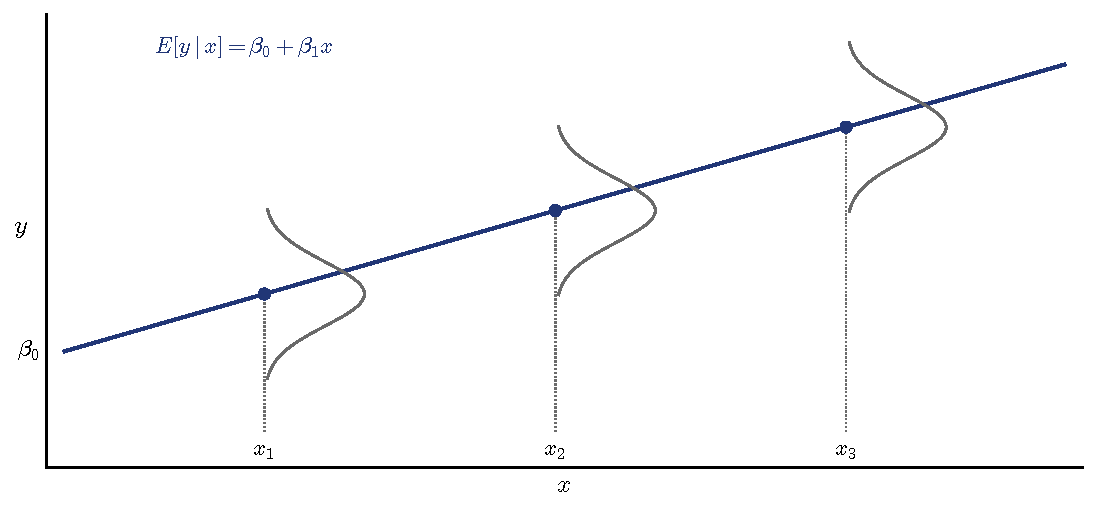
\includegraphics[width=.82\linewidth]{conditional_means.pdf}
\caption{不同 $x$ 取值下的总体条件均值。侧面的曲线表示条件分布；本图为教学示意，不是实际观测数据。}
\label{fig:conditional-means}
\end{figure}
\paragraph{普通最小二乘法（OLS）。}
\textbf{拟合回归线}，亦称样本回归线，为
\begin{equation}\label{eq:fitted-simple}
\hat y_i=\hat\beta_0+\hat\beta_1x_i,
\qquad \hat\beta_0=\bar y-\hat\beta_1\bar x.
\end{equation}
若样本中的 $x$ 存在变异，则
\begin{equation}\label{eq:simple-slope}
\hm{\hat\beta_1=
\frac{\sum_i(x_i-\bar x)(y_i-\bar y)}{\sum_i(x_i-\bar x)^2}
=\frac{\Cov_n(x,y)}{\Var_n(x)}
=r_{xy}\frac{s_y}{s_x}}.
\end{equation}
其中 $r_{xy}=\Cov_n(x,y)/(s_xs_y)$。分子与分母采用一致的协方差归一化约定。\corr{slope-correlation}

\textbf{斜率。}其他条件不变时，$x$ 增加一个单位，\hy{与 $y$ 的预测值增加 $\hat\beta_1$ 个单位相关联}。
\blue{原稿例式：$y=\beta_0+\beta_1x+\beta_2z+\beta_3w+u$；若 $z,w$ 遗漏，简单回归系数可能把它们的影响一并算入。}

\red{相关不等于因果。}缺少合理的数据生成过程和识别假设时，应使用“相关联”或“相关”等措辞，而不应使用“导致”“使得”等因果表述。若模型具有可辩护的结构性、外生性及因果识别条件，才可进一步解释为因果效应。\corr{causality}

\textbf{截距。}$x=0$ 时，$y$ 的拟合值为 $\hat\beta_0$；在式 \eqref{eq:prf} 成立时，$x=0$ 处的总体条件均值为 $\beta_0$。若零不在观测范围或可行范围内，这一解释可能只是外推。

拟合线取决于样本；总体回归线则固定但未知。原稿中薪酬与净资产收益率的例式保留为
\[\widehat{\mathrm{salary}}=963.191+18.501\,\mathrm{roe}.\]
\begin{figure}[htbp]
\centering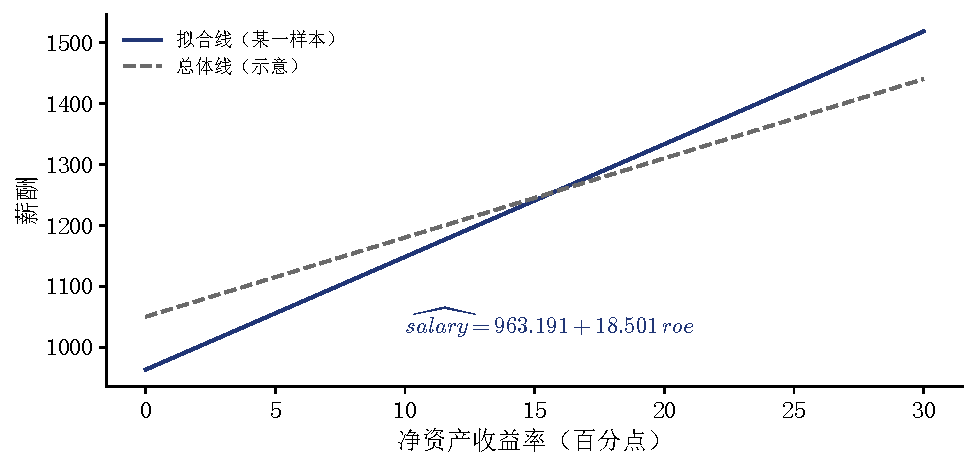
\includegraphics[width=.8\linewidth]{fitted_population.pdf}
\caption{拟合回归线与总体回归线的比较，沿用原稿中薪酬与净资产收益率的示意。总体线仅作示意，并非另行估计的基准。}
\label{fig:fitted-population}
\end{figure}

\subsection{例题：单位与百分点}
\sourcepage{2}{3}{2/3}
\begin{example}[小时工资：注意单位]\label{ex:wage-units}
原题将小时工资的单位规定为\hy{千美元}，教育年限的单位为年：
\[\wage=\beta_0+\beta_1\educ+u,\qquad
\widehat{\wage}=-0.9+0.54\educ.\]
安森每小时挣 6 美元，受教育年限为 12 年。若保持未观测因素不变，当其受教育年限变为 16 年时，模型给出的情景工资是多少？
\begin{align*}
\widehat{\wage}_{12}&=-0.9+0.54(12)=5.58\quad\text{（千美元/小时）},\\
\hat u_{\text{安森}}&=0.006-5.58=-5.574,\\
\Delta\widehat{\wage}&=0.54(16-12)=2.16\quad\text{（千美元/小时）},\\
\widehat{\wage}_{16}&=-0.9+0.54(16)=7.74.
\end{align*}
在本题的模型情景中，若将拟合残差保持不变，则
\[\wage_{16}^{\text{情景}}=7.74-5.574=2.166,
\qquad\text{即每小时 }2{,}166\text{ 美元}.\]
等价地，
\[\hp{情景工资 = 原实际工资 + 模型给出的变化量},\]
\[\$6+(\$0.54\times10^3\times4)=\$2{,}166.\]
\added{数值异常大，是因为原稿明确采用了\emph{千美元}的单位；本笔记没有擅自将单位改成美元。固定某个人的误差或拟合残差，只是一项假设情景，不代表已经识别出的个体反事实，也不能保证其未来的实际工资。}\corr{wage-counterfactual}
\end{example}

\begin{exercise}[竞选支出]\label{ex:election}
\[\widehat{\mathrm{voteA}}=26.81+0.464\,\mathrm{shareA}.\]
其中，$\mathrm{voteA}$ 表示候选人 A 的得票百分比；$\mathrm{shareA}$ 表示 A 的竞选支出占两位候选人总支出的百分比。支出占比每增加一个\hy{百分点}，与预测得票率增加 0.464 个百分点相关联。
\begin{enumerate}
\item 若支出占比为 $40\%$，应代入 $40$，而不是 $0.40$：
\[\widehat{\mathrm{voteA}}=26.81+0.464(40)=\hm{45.37\%}.\]
若 A 完全不支出，拟合值为 $26.81$；若 A 承担全部支出，则为 $26.81+0.464(100)=73.21$。这些是拟合线给出的预测，不能保证选举结果。
\item 若候选人 B 支出 20 亿美元，A 至少需要达到怎样的支出门槛，才能使\emph{预测}得票率超过 $50\%$？
\begin{align*}
26.81+0.464\,\mathrm{shareA}&>50,\\
\mathrm{shareA}&>\frac{23.19}{0.464}=49.978448\ldots.
\end{align*}
\added{令 $A$ 表示以十亿美元为单位的支出。由于 $\mathrm{shareA}=100A/(A+2)$，有
\[A>\frac{2(49.978448\ldots)}{100-49.978448\ldots}
=1.9982766\ldots\ \text{十亿美元}.\]
严格不等式给出的是支出门槛；在连续支出范围内，该门槛并不是能够取到的最小值。此回归不能保证实际获胜。}\corr{election}
\end{enumerate}
\end{exercise}

\section{多元 OLS 的解释}
\sourcepage{2}{4}{2/4}
\label{sec:multiple-interpretation}
总体模型与拟合方程分别为
\begin{align}
y&=\beta_0+\beta_1x_1+\cdots+\beta_kx_k+u,\label{eq:multiple-model}\\
\hat y&=\hat\beta_0+\hat\beta_1x_1+\cdots+\hat\beta_kx_k.\label{eq:multiple-fitted}
\end{align}
对一个给定的拟合方程，有
\[\hm{\Delta\hat y=\hat\beta_1\Delta x_1+\cdots+\hat\beta_k\Delta x_k}.\]
保持其余 $x_j$ 全部不变，得到
\[\Delta\hat y=\hat\beta_\ell\Delta x_\ell,
\qquad\frac{\Delta\hat y}{\Delta x_\ell}=\hat\beta_\ell.
\]
\textbf{偏效应。}在总体模型中，保持其余回归变量\emph{以及} $u$ 不变时，$\beta_\ell=\Delta y/\Delta x_\ell$；在 ZCM 下，它也是 $\E[y\mid x_1,\ldots,x_k]$ 对该变量的偏斜率。\corr{notation}
\[\hy{$\E[u\mid x_1,\ldots,x_k]=0$}.\]
将其他解释变量纳入回归，就可以在拟合比较中保持其观测值不变。\blue{不需要 $x_\ell$ 与其他 $x_j$ 互不相关；只需避免完全共线性，才能区分各自系数。}

\begin{example}[大学平均绩点]\label{ex:gpa}
\[\widehat{\colGPA}=1.29+0.453\hsGPA+0.0094\ACT.\]
原稿给定的范围为：大学平均绩点 $\colGPA$ 为 $0$--$4$，高中平均绩点 $\hsGPA$ 为 $1$--$4$，ACT 考试分数为 $0$--$36$。
\begin{description}
\item[高中绩点。]保持 ACT 分数及其他因素不变，高中平均绩点每提高 1 分，与大学平均绩点的预测值提高 0.453 分相关联。
\item[ACT 分数。]保持高中平均绩点及其他因素不变，ACT 分数每提高 1 分，与大学平均绩点的预测值提高 0.0094 分相关联。
\item[截距。]高中绩点与 ACT 分数都为零时，大学平均绩点的拟合值为 $1.29$。\red{高中绩点为零超出了题定范围}，因此这只是外推，并非对某个已观测群体的预测。
\end{description}
\begin{enumerate}
\item 若 ACT 分数固定，高中绩点从 $3.5$ 升至 $3.6$，则
\[\Delta\widehat{\colGPA}=(3.6-3.5)(0.453)=0.0453.\]
\item 安森的高中绩点为 $3.5$、ACT 为 $30$；贝蒂的高中绩点为 $3.0$、ACT 为 $36$：
\begin{align*}
\widehat{\colGPA}_{A}&=1.29+0.453(3.5)+0.0094(30)=3.1575,\\
\widehat{\colGPA}_{B}&=1.29+0.453(3.0)+0.0094(36)=2.9874.
\end{align*}
\item 若安森的实际大学绩点为 $3.3$，能否推断贝蒂的实际绩点？不能。\blue{每个人的 $u$ 不同，不能由一个人的实际值推出另一个人的实际值。}安森在本样本中的残差为 $3.3-3.1575=0.1425$；贝蒂的残差未知。
\end{enumerate}
\end{example}


\section{控制变量与 FWL 定理}
\sourcepage{2}{5}{2/5}
\label{sec:fwl-week2}
\subsection{为什么引入控制变量？}
假设我们关心教育年限 $x_1$ 对工资 $y$ 的影响，而能力 $x_2$ 也会影响工资：
\[y=\beta_0+\beta_1x_1+\beta_2x_2+u.\]
若遗漏能力，短方程 $y=\tilde\beta_0+\tilde\beta_1x_1+v$ 可能将能力的影响归到教育上。当能力既影响工资又与教育相关时，这就涉及\hp{遗漏变量偏误}。

“控制”可以从两个角度理解：
\begin{enumerate}
\item \hy{保持不变}：保持 $x_2$ 固定，比较 $x_1$ 的变化。
\item \hy{剔除线性影响}：先移除能够由 $x_2$ 线性解释的部分，再解读 $x_1$ 的系数。
\end{enumerate}
\blue{二者描述的是同一个多元回归系数；FWL 将“排除其他变量的线性影响”写成可计算的步骤。}

\subsection{将回归变量残差化}
在样本中，先将 $x_1$ 对常数项与 $x_2$ 回归：
\begin{equation}\label{eq:fwl-x}
x_{1i}=\hat\delta_0+\hat\delta_1x_{2i}+\hat r_{1i}.
\end{equation}
残差 $\hat r_{1i}$ 是 $x_{1i}$ 中\hy{不能由 $x_2$ 线性解释的部分}，并满足
\[\sum_i\hat r_{1i}=0,\qquad\sum_i x_{2i}\hat r_{1i}=0.\]
再将 $y_i$ 对常数项与 $\hat r_{1i}$ 回归，其斜率恰好等于原多元 OLS 中 $x_1$ 的系数：
\begin{equation}\label{eq:fwl-one-sided}
\hm{\hat\beta_1=
\frac{\Cov_n(\hat r_1,y)}{\Var_n(\hat r_1)}
=\frac{\sum_i\hat r_{1i}y_i}{\sum_i\hat r_{1i}^2}}.
\end{equation}
因此，$\hat\beta_1$ 描述的是：剔除 $x_1$ 与 $x_2$ 的线性关系后，$x_1$ 的剩余变化与 $y$ 之间的拟合关系。\blue{将 $x_1$ 对控制变量回归，留下不被它们线性解释的部分。}

\added{标准的双侧 FWL 回归还需将 $y$ 对 $(1,x_2)$ 回归，得到 $\hat r_{yi}$，再将 $\hat r_y$ 对 $\hat r_1$ 作无截距回归。所得斜率\emph{与残差}均和完整模型相同。原稿中的单侧回归给出相同斜率，但通常不会给出相同的回归残差。}\corr{fwl-residual}

\subsection{一般情形}
对 $y=\beta_0+\beta_1x_1+\cdots+\beta_kx_k+u$，将 $x_1$ 对 $(1,x_2,\ldots,x_k)$ 回归：
\[x_{1i}=\hat\delta_0+\hat\delta_2x_{2i}+\cdots+\hat\delta_kx_{ki}+\hat r_{1i}.\]
将 $y_i$ 对 $\hat r_{1i}$ 与常数项回归；也可将经过相应残差化的 $y_i$ 对 $\hat r_{1i}$ 作无截距回归。只要残差变异为正，式 \eqref{eq:fwl-one-sided} 仍成立。更多细节及原稿重复的推导保留在\hyperref[sec:fwl-week3]{第 3 周}和\hyperref[sec:fwl-week4]{第 4 周}。

\section{简单回归与多元回归的斜率比较}
\sourcepage{2}{6}{2/6}
\label{sec:short-long-week2}
增加一个控制变量时，它必须与原回归变量不相关吗？\red{不用！}控制变量与原变量相关，恰恰是简单与多元回归斜率经常不同的原因。但控制变量应适合所研究的因果或预测问题；加入它并不自动消除偏误。

考虑以下总体方程：
\begin{align*}
y&=\beta_0+\beta_1x_1+\beta_2x_2+u,\\
x_2&=\delta_0+\delta_1x_1+\varepsilon.
\end{align*}
第二个方程是总体线性投影，满足 $\E[\varepsilon]=\E[x_1\varepsilon]=0$。若 $\E[u\mid x_1,x_2]=0$，代入可得
\begin{align*}
y&=\beta_0+\beta_1x_1+\beta_2(\delta_0+\delta_1x_1+\varepsilon)+u\\
 &=\underbrace{(\beta_0+\beta_2\delta_0)}_{\tilde\beta_0}
  +\underbrace{(\beta_1+\beta_2\delta_1)}_{\tilde\beta_1}x_1
  +\underbrace{(u+\beta_2\varepsilon)}_{v}.
\end{align*}
因此，短模型的总体投影斜率为
\begin{equation}\label{eq:population-ovb}
\hm{\tilde\beta_1=\beta_1+\beta_2\delta_1}.
\end{equation}
这是\emph{总体投影系数}之间的关系，不能写成估计量与固定总体参数之间的相等关系。\corr{ovb-levels}

\paragraph{两个斜率何时相同？}
在含两个回归变量的情形中，$\tilde\beta_1=\beta_1$ 当且仅当 $\beta_2\delta_1=0$：
\begin{enumerate}
\item $\beta_2=0$：$x_2$ 对 $y$ 的偏效应为零；即使 $x_1$ 与 $x_2$ 相关，两个总体斜率仍相同。
\item $\delta_1=0$：$x_1$ 与 $x_2$ 在总体中不相关。
\end{enumerate}
\added{对于具体样本中的 OLS 系数，精确的样本恒等式为
\[\hat{\tilde\beta}_1=\hat\beta_1+\hat\beta_2\hat\delta_1.\]
因此，若 $\hat\beta_2=0$，或\emph{样本}辅助回归斜率 $\hat\delta_1=0$，两个样本斜率相同。总体系数为零，并不强制其样本估计值恰好为零。}

\begin{example}[平均绩点：控制变量改变系数解释]\label{ex:gpa-short-long}
比较以下经过舍入的拟合方程：
\begin{align*}
\widehat{\colGPA}&=1.29+0.453\hsGPA+0.0094\ACT,\\
\widehat{\colGPA}&\simeq2.40+0.0271\ACT
                       &&\text{（仅含 ACT）},\\
\widehat{\hsGPA}&\simeq2.46+0.039\ACT,\\
\widehat{\colGPA}&\simeq1.41+0.482\hsGPA
                       &&\text{（仅含高中绩点）}.
\end{align*}
以 ACT 为例，以下舍入数值的运算体现了总体或样本方程相互代入的直觉：
\[1.29+0.453(2.46)=2.40438,\qquad
0.0094+0.453(0.039)=0.027067\simeq0.0271.\]
仅含高中绩点的斜率与其多元回归斜率较接近，部分原因是 ACT 的偏回归系数较小。\blue{小的遗漏系数只有与辅助回归系数的大小一起看，才说明偏差是否小。}以上方程均为原稿中经过舍入的例子，并非重新估计的实证结果。
\end{example}

\section{计量单位与函数形式}
\sourcepage{2}{7}{2/7}
\label{sec:units}
\subsection{改变因变量的计量单位}
从 $y=\beta_0+\beta_1x+u$ 出发。若 $y'=cy$ 且 $c\ne0$，则
\[y'=c\beta_0+c\beta_1x+cu.\]
因此，
\[\hy{$\beta'_0=c\beta_0$},\qquad
\hy{$\beta'_1=c\beta_1$},\qquad u'=cu,\qquad\Delta y'=c\Delta y.\]
例如，从美元换算为千美元时，$c=1/1000$。
样本 OLS 的推导为
\begin{align*}
\hat\beta'_1
 &=\frac{\Cov_n(x,y')}{\Var_n(x)}
 =\frac{\Cov_n(x,cy)}{\Var_n(x)}
 =c\hat\beta_1,\\
\hat\beta'_0
 &=\bar y'-\hat\beta'_1\bar x
 =c\bar y-c\hat\beta_1\bar x=c\hat\beta_0.
\end{align*}
在 ZCM 下，$x=0$ 处的截距解释变为
\[\E[y'\mid x=0]=c\beta_0=\beta'_0.\]
\red{这里必须写条件均值；通常不能写成 $\beta_0=\E[y]$。}一般地，当 $\E[u]=0$ 时，$\E[y]=\beta_0+\beta_1\E[x]$。\corr{unit-intercept}

\subsection{改变回归变量的计量单位}
若 $x'=cx$ 且 $c\ne0$，则
\[y=\beta_0+\frac{\beta_1}{c}x'+u,\qquad
\hy{$\beta'_0=\beta_0$},\quad\hy{$\beta'_1=\beta_1/c$}.\]
$x'=0$ 时也有 $x=0$，因此截距不变。对拟合系数，有
\begin{align*}
\hat\beta'_1
 &=\frac{\Cov_n(x',y)}{\Var_n(x')}
 =\frac{c\Cov_n(x,y)}{c^2\Var_n(x)}
 =\frac{\hat\beta_1}{c},\\
\hat\beta'_0&=\bar y-\frac{\hat\beta_1}{c}(c\bar x)=\hat\beta_0.
\end{align*}
相应的拟合均值恒等式为 $\bar y=\hat\beta'_0+\hat\beta'_1\bar x'$。

\section{水平值与对数模型}
\sourcepage{2}{8}{末页}
\label{sec:logs}
\blue{水平值对应单位变化；对数对应相对或百分比变化。}以下对数均为自然对数，要求真数为正。比较时始终保持误差与其他回归变量不变。普通有限百分比变化记为 $\%\Delta x=100\Delta x/x_0$ 和 $\%\Delta y=100\Delta y/y_0$。

\subsection{水平值—水平值模型}
\[y=\beta_0+\beta_1x+u,\qquad
\hm{\Delta y=\beta_1\Delta x}.\]
$x$ 每增加一个单位，对应 $y$ 增加 $\beta_1$ 个单位。

\subsection{水平值—对数模型}
\[y=\beta_0+\beta_1\ln x+u,\qquad
\frac{dy}{d\ln x}=\beta_1,\qquad
dy=\beta_1\frac{dx}{x}.\]
对于较小的变化，
\[\hm{\Delta y\approx\frac{\beta_1}{100}\,\%\Delta x}.\]
$x$ 增加百分之一，与 $y$ 大约增加 $\beta_1/100$ 个单位相对应。
\added{对于有限变化，模型的精确关系为 $\Delta y=\beta_1\ln(x_1/x_0)$。当 $x$ 增加 $1\%$ 时，变化量为 $\beta_1\ln(1.01)$，并不恰好等于 $\beta_1/100$。}\corr{logs}

\subsection{对数—水平值模型}
\[\ln y=\beta_0+\beta_1x+u,\qquad
\frac{d\ln y}{dx}=\beta_1=\frac{1}{y}\frac{dy}{dx}.\]
因此，$\beta_1$ 是以小数表示的半弹性，且
\[\hm{\%\Delta y\approx100\beta_1\Delta x}.\]
$x$ 每增加一个单位，对应 $y$ 的变化率约为 $100\beta_1\%$。
\added{对于有限的 $\Delta x$，在保持误差不变时，精确关系为
\[\%\Delta y=100\bigl(e^{\beta_1\Delta x}-1\bigr).\]
将 $\E[\ln y\mid x]$ 取指数，一般不等于 $\E[y\mid x]$；若要解释水平值的条件均值，还需要进行反变换调整。}\corr{logs}

\subsection{对数—对数模型}
\[\ln y=\beta_0+\beta_1\ln x+u,\qquad
\hm{\beta_1=\frac{d\ln y}{d\ln x}
=\frac{dy/y}{dx/x}}.\]
$\beta_1$ 是弹性。对于较小的变化，
\[\%\Delta y\approx\beta_1\,\%\Delta x.\]
$x$ 增加百分之一，对应 $y$ 大约变化 $\beta_1\%$。
\added{对于普通有限百分比变化 $p=\%\Delta x$，
\[\%\Delta y=100\left[\left(1+\frac p{100}\right)^{\beta_1}-1\right].\]
微分形式的弹性关系是精确的；将微分替换为任意有限变化，则属于近似。}\corr{logs}

\subsection*{本章小结}
\addcontentsline{toc}{subsection}{本章小结}
\begin{itemize}
\item 拟合斜率描述预测上的关联；因果解释还需要恰当的模型与研究设计。
\item 多元 OLS 在比较中保持已纳入的控制变量不变；FWL 通过残差化提取同一个斜率。
\item 单位变化会相应缩放系数。解释对数模型时，须明确区分精确关系与百分比近似。
\end{itemize}

\chapter{拟合优度}
\label{ch:week3}
\section{简单回归的情形}
\sourcepage{3}{1}{3/1}
\label{sec:simple-properties}
本章区分拟合值与残差，并介绍判定系数 $R^2$。
\[y_i=\beta_0+\beta_1x_i+u_i,\qquad
\hat y_i=\hat\beta_0+\hat\beta_1x_i.\]
\begin{definition}[误差与残差]
\[\underbrace{u_i=y_i-\beta_0-\beta_1x_i}_{\text{总体误差}},\qquad
\underbrace{\hat u_i=y_i-\hat y_i=y_i-\hat\beta_0-\hat\beta_1x_i}_{\text{OLS 残差}}.\]
完成拟合后，残差可以计算并观测；总体误差则依赖未知的总体参数。
\end{definition}

\subsection{含截距 OLS 的三个样本性质}
\paragraph{性质一：残差的样本均值为零。}
OLS 使 $Q(b_0,b_1)=\sum_i(y_i-b_0-b_1x_i)^2$ 最小。在最优点，
\[\left.\frac{\partial Q}{\partial b_0}\right|_{\hat\beta}
=-2\sum_{i=1}^n\hat u_i=0
\quad\Longrightarrow\quad\hm{\sum_i\hat u_i=0},\quad\bar{\hat u}=0.\]

\paragraph{性质二：残差与 $x$ 在样本中正交。}
关于斜率的一阶条件为
\[\left.\frac{\partial Q}{\partial b_1}\right|_{\hat\beta}
=-2\sum_i x_i\hat u_i=0.\]
因此，
\begin{align*}
\Cov_n(x,\hat u)
&=\frac1n\sum_i(x_i-\bar x)(\hat u_i-\bar{\hat u})\\
&=\frac1n\left(\sum_i x_i\hat u_i-\bar x\sum_i\hat u_i\right)=0.
\end{align*}
\hy{残差与 $x$ 在样本中不相关}。若某个变量的方差为零，相关系数本身未定义；但正交关系仍成立。

每个观测可分解为 $y_i=\hat y_i+\hat u_i$，且拟合值与残差在样本中正交：
\[\sum_i\hat y_i\hat u_i
=\hat\beta_0\sum_i\hat u_i+\hat\beta_1\sum_i x_i\hat u_i=0.\]

\paragraph{总体矩条件：另一个层面的结论。}
总体矩条件可以利用迭代期望法则得到。若 $\E[u\mid x]=0$ 且所需可积性条件成立，则
\[\E[u]=\E\{\E[u\mid x]\}=0,\qquad
\E[xu]=\E\{x\E[u\mid x]\}=0.\]
\red{这些总体限制不能用来证明样本正规方程。}即使总体外生性假设不成立，上述样本恒等式仍直接来自残差平方和的最小化。\corr{sample-population}

\paragraph{性质三：样本均值点位于拟合线上。}
由于 $\hat\beta_0=\bar y-\hat\beta_1\bar x$，有
\[\hm{\bar y=\hat\beta_0+\hat\beta_1\bar x}.\]
也可以对 $\hat y_i=\hat\beta_0+\hat\beta_1x_i$ 取样本平均：
\[\bar{\hat y}=\frac1n\sum_i\hat y_i=\hat\beta_0+\hat\beta_1\bar x,
\qquad\bar y=\bar{\hat y}+\bar{\hat u}=\bar{\hat y}.\]
对应的\emph{总体}结论是：若 $\E[u]=0$，则 $\E[y]=\beta_0+\beta_1\E[x]$。这里应使用总体参数，而不是带帽的拟合系数。\corr{sample-population}

\section{平方和与拟合优度}
\sourcepage{3}{2}{3/2}
\label{sec:ss-decomposition}
\begin{definition}[总平方和、解释平方和与残差平方和]
\begin{align}
\TSS&=\sum_{i=1}^n(y_i-\bar y)^2=(n-1)s_y^2,\label{eq:tss}\\
\ESS&=\sum_{i=1}^n(\hat y_i-\bar y)^2,\label{eq:ess}\\
\RSS&=\sum_{i=1}^n\hat u_i^2=\sum_{i=1}^n(y_i-\hat y_i)^2.\label{eq:rss}
\end{align}
其中，$s_y^2=\sum_i(y_i-\bar y)^2/(n-1)$ 为样本方差。
\end{definition}
\blue{TSS：$y$ 围绕均值的总波动；ESS：回归线所解释的波动；RSS：回归未解释的残差波动。}本笔记用 ESS 表示\emph{解释}平方和；其他教材有时采用不同的缩写约定。

\begin{theorem}[平方和分解]
对于含截距的 OLS，
\begin{equation}\label{eq:anova}
\hm{\TSS=\ESS+\RSS}.
\end{equation}
\end{theorem}
\begin{proof}
由于 $y_i-\bar y=(\hat y_i-\bar y)+\hat u_i$，有
\begin{align*}
\TSS
&=\sum_i\bigl[(\hat y_i-\bar y)+\hat u_i\bigr]^2\\
&=\sum_i(\hat y_i-\bar y)^2+\sum_i\hat u_i^2
  +2\sum_i\hat u_i(\hat y_i-\bar y).
\end{align*}
因为 $\sum_i\hat u_i\hat y_i=0$ 且 $\sum_i\hat u_i=0$，交叉项为零，故式 \eqref{eq:anova} 成立。
\end{proof}
\blue{OLS 的目标是使 $\sum_i\hat u_i^2$ 最小，而不是使 $\sum_i\hat u_i$ 最小；后者为零来自截距的一阶条件。}

\subsection[判定系数的定义与解释]{判定系数 $R^2$ 的定义与解释}
当 $\TSS>0$ 时，定义
\begin{equation}\label{eq:r2}
\hm{R^2=\frac{\ESS}{\TSS}=1-\frac{\RSS}{\TSS}\in[0,1]}.
\end{equation}
\textbf{解释。}$R^2$ 衡量回归中各变量所解释的 \hy{$y$ 的样本波动占比}。例如，$R^2=0.85$ 表示因变量样本波动的 $85\%$ 可以由该回归解释。

若所有观测点都位于拟合线上，即 $y_i=\hat y_i$，则 $\RSS=0$、$\TSS=\ESS$，并且 $R^2=1$。这就是完全拟合。
\begin{figure}[htbp]
\centering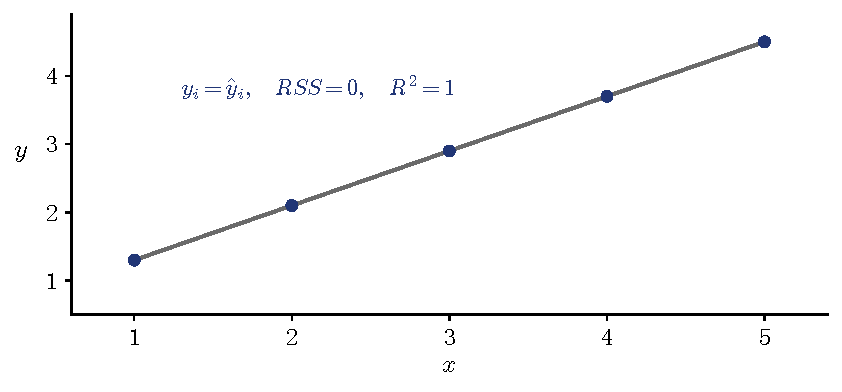
\includegraphics[width=.68\linewidth]{perfect_fit.pdf}
\caption{原稿中的完全拟合情形：全部示意观测点均落在拟合线上。}
\label{fig:perfect-fit}
\end{figure}

\subsection{相关系数平方的解释}
若 $y$ 与 $\hat y$ 的样本方差均为正，则
\begin{equation}\label{eq:r2-correlation}
R^2=\Corr_n(y,\hat y)^2
=\frac{\left[\sum_i(y_i-\bar y)(\hat y_i-\bar y)\right]^2}
{\left[\sum_i(y_i-\bar y)^2\right]\left[\sum_i(\hat y_i-\bar y)^2\right]}.
\end{equation}
利用 $y_i=\hat y_i+\hat u_i$、$\bar y=\bar{\hat y}$ 以及样本正交性，可得
\[\Cov_n(y,\hat y)=\Var_n(\hat y),\qquad
\Corr_n(y,\hat y)^2=\frac{\Var_n(\hat y)}{\Var_n(y)}=\frac{\ESS}{\TSS}.
\]
\added{若所有 $y_i$ 都相同，则 TSS 为零，此处的中心化 $R^2$ 未定义。若 $\hat y$ 为常数而 $y$ 存在变异，则 $R^2=0$，但 $\Corr_n(y,\hat y)$ 未定义；此时不能使用相关系数平方的公式进行计算。}\corr{r2-degenerate}

\subsection{图形比较}
\sourcepage{3}{3}{3/3}
\begin{figure}[htbp]
\centering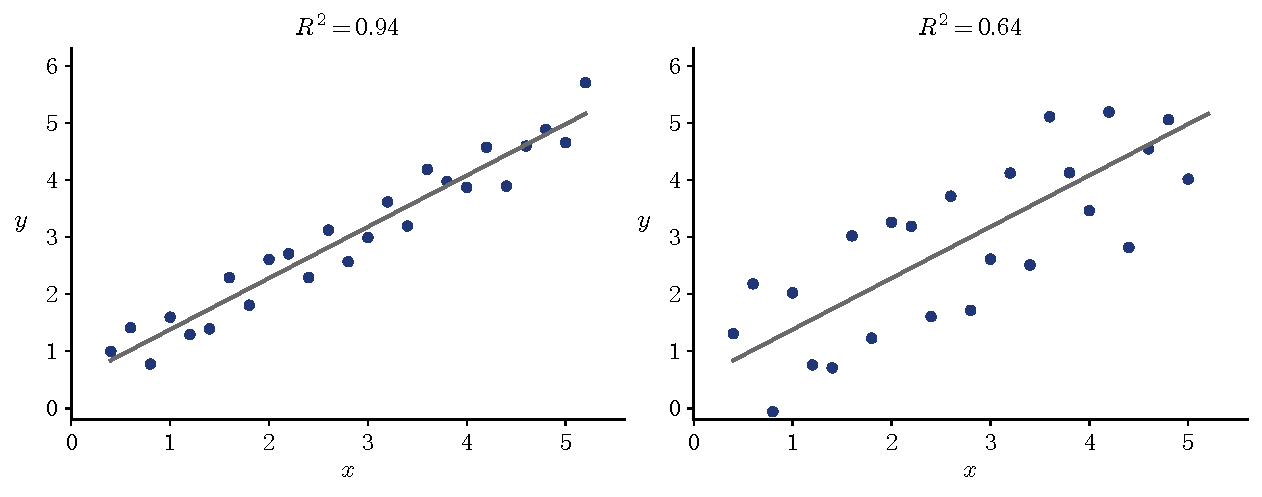
\includegraphics[width=.95\linewidth]{r_squared_comparison.pdf}
\caption{采用原稿中 $R^2=0.94$ 与 $R^2=0.64$ 的两组示意样本。图中的数值由新生成的观测点及其拟合线实际计算。}
\label{fig:r2-comparison}
\end{figure}
较高的 $R^2$ 对应较小的残差\emph{占比} $\RSS/\TSS$；较低的 $R^2$ 则对应较大的残差占比。\blue{较低时，仅靠当前回归变量，对 $y$ 的样本波动解释得较少。}不能只凭 $R^2$，就跨不同样本或不同因变量单位比较 RSS 的绝对大小。\corr{r2-rss}

\section{多元回归的情形}
\label{sec:multiple-properties}
模型、拟合值与残差分别为
\begin{align*}
y_i&=\beta_0+\beta_1x_{1i}+\cdots+\beta_kx_{ki}+u_i,\\
\hat y_i&=\hat\beta_0+\hat\beta_1x_{1i}+\cdots+\hat\beta_kx_{ki},\\
\hat u_i&=y_i-\hat y_i.
\end{align*}
前述三个样本性质可推广到多元回归。

\paragraph{性质一：残差均值为零。}
令 $Q(b)=\sum_i(y_i-b_0-\sum_{j=1}^k b_jx_{ji})^2$，则
\[\left.\frac{\partial Q}{\partial b_0}\right|_{\hat\beta}
=-2\sum_i\hat u_i=0
\quad\Longrightarrow\quad\sum_i\hat u_i=0,\quad\bar{\hat u}=0.\]

\paragraph{性质二：残差与每个已纳入的回归变量在样本中正交。}
对于每个 $j=1,\ldots,k$，
\[\left.\frac{\partial Q}{\partial b_j}\right|_{\hat\beta}
=-2\sum_i x_{ji}\hat u_i=0
\quad\Longrightarrow\quad\hm{\sum_i x_{ji}\hat u_i=0}.\]
结合截距的一阶条件，得到 $\Cov_n(x_j,\hat u)=0$。

\paragraph{性质三：样本均值向量位于拟合超平面上。}
对 $y_i=\hat y_i+\hat u_i$ 取平均，得 $\bar y=\bar{\hat y}$，因此
\begin{align*}
\bar y
&=\frac1n\sum_i\left(\hat\beta_0+\hat\beta_1x_{1i}+\cdots+\hat\beta_kx_{ki}\right)\\
&=\hm{\hat\beta_0+\hat\beta_1\bar x_1+\cdots+\hat\beta_k\bar x_k}.
\end{align*}
采用与式 \eqref{eq:anova} 相同的证明，可知含截距的多元 OLS 仍满足 TSS $=$ ESS $+$ RSS，并适用同一个 $R^2$ 公式。

\section[增加回归变量与调整判定系数]{增加回归变量与调整 $R^2$}
\sourcepage{3}{4}{3/4}
\label{sec:adjusted-r2}
回顾以下定义：
\[\TSS=\sum_i(y_i-\bar y)^2,\quad
\ESS=\sum_i(\hat y_i-\bar y)^2,\quad
\RSS=\sum_i(y_i-\hat y_i)^2.\]
若增加回归变量，$R^2$ 会怎样变化？
\begin{itemize}
\item 对于\emph{相同观测和同一因变量}，若两个嵌套模型均含截距，新模型最小化后的 RSS 不会大于旧模型：将新增系数设为零，就可以复现旧模型的拟合。
\item 因此，$R^2$ \hy{不会下降}，但可能完全不变。不断加入变量可能导致样本内过拟合。\corr{r2-monotonic}
\item $R^2$ 不能建立因果关系。高 $R^2$ 不一定意味着因果，低 $R^2$ 也不能排除因果。
\end{itemize}

\subsection{自由度调整}
若不计截距有 $k$ 个回归变量，且 $n>k+1$、$\TSS>0$，则
\begin{equation}\label{eq:adjusted-r2}
\hm{\bar R^2=1-\frac{\RSS/(n-k-1)}{\TSS/(n-1)}
=1-\frac{n-1}{n-k-1}(1-R^2)}.
\end{equation}
\blue{自由度修正：增加回归变量会受到惩罚，RSS 的减少必须足以补偿损失的自由度。}
\begin{itemize}
\item $\bar R^2$ 对回归变量个数施加惩罚，因此增加变量时可能下降。
\item 若残差均方超过仅含均值模型的基准均方，它可以为负。
\item $\bar R^2$ 上升，只说明在此调整标准下，样本内拟合改善足够大；这并不证明变量具有实质重要性或因果作用。
\end{itemize}
\added{增加 $q$ 个回归变量时，$\bar R^2$ 上升当且仅当
\[
\frac{(\RSS_{\text{旧}}-\RSS_{\text{新}})/q}{\RSS_{\text{新}}/(n-k_{\text{新}}-1)}>1,
\]
其中假设分母为正。这是描述性的偏 $F$ 统计量门槛 1，并非常规显著性检验的临界值。}\corr{adjusted-meaning}

\begin{example}[平均绩点：原稿中的取舍]
使用原稿给出的舍入数值，且 $n=141$：
\begin{align*}
\text{仅含高中绩点：}\quad &R^2=0.172,\quad k=1,\\
&\bar R^2=1-\frac{140}{139}(1-0.172)=0.166043\ldots,\\
\text{高中绩点与 ACT：}\quad &R^2=0.176,\quad k=2,\\
&\bar R^2=1-\frac{140}{138}(1-0.176)=0.164058\ldots.
\end{align*}
加入 ACT 后，普通 $R^2$ 上升，而调整 $R^2$ 略微下降。这些结果由原稿中经过舍入的输入数值计算；超出输入精度的小数位仅表示算术计算精度。
\end{example}

\paragraph{注意（保留原稿的三点提醒）.}
\begin{enumerate}
\item $R^2$ 描述样本拟合：高 $R^2\ne$ 因果，低 $R^2\ne$ 没有因果。
\item 加入变量可能造成过拟合；调整 $R^2$ 虽引入惩罚，却不能单独保证样本外表现。
\item 良好的拟合并不自动消除遗漏变量偏误。
\end{enumerate}


\section{过原点回归与去均值}
\sourcepage{3}{5}{3/5}
\label{sec:rto}
回顾\emph{仅含截距}的回归：$\hat\beta_0=\bar y$，证明见下文。这一恒等式不适用于任意含 $x$ 的回归。

\subsection{过原点回归（RTO）}
有时模型被限制为经过原点。例如，某个生产关系假定投入为零时，期望产出也为零。这是额外的建模限制，并不是生产数据自动具备的性质。
\[y_i=\beta_1^{\rm RTO}x_i+u_i,\qquad
\hat y_i=\check\beta_1x_i,\qquad\check u_i=y_i-\hat y_i.\]
此处使用倒帽记号，区分这一拟合斜率及其残差与含截距 OLS 的对应量。最小化
\[Q(b_1)=\sum_i(y_i-b_1x_i)^2\]
可得一阶条件
\[\sum_i x_i(y_i-\check\beta_1x_i)=0
\quad\Longrightarrow\quad
\hm{\check\beta_1=\frac{\sum_i x_iy_i}{\sum_i x_i^2}}
\quad\text{其中 }\sum_i x_i^2>0.
\]

\subsection{去均值后可复现含截距回归的斜率}
定义 $A_i=y_i-\bar y$、$B_i=x_i-\bar x$。将 $A_i$ 对 $B_i$ 作过原点回归，其斜率为
\[\frac{\sum_iB_iA_i}{\sum_iB_i^2}
=\frac{\sum_i(x_i-\bar x)(y_i-\bar y)}{\sum_i(x_i-\bar x)^2}
=\hat\beta_1.\]
因此，对\emph{去均值}变量作无截距回归，可以复现普通\emph{含截距} OLS 的斜率。这不意味着未经中心化的无截距回归也具有相同斜率。\corr{demeaning}

对于含截距的 OLS，
\[y_i-\bar y=\hat\beta_1(x_i-\bar x)+\hat u_i.\]
\blue{截距项使回归线经过样本均值 $(\bar x,\bar y)$；去均值相当于平移坐标，不改变斜率。}
\begin{figure}[htbp]
\centering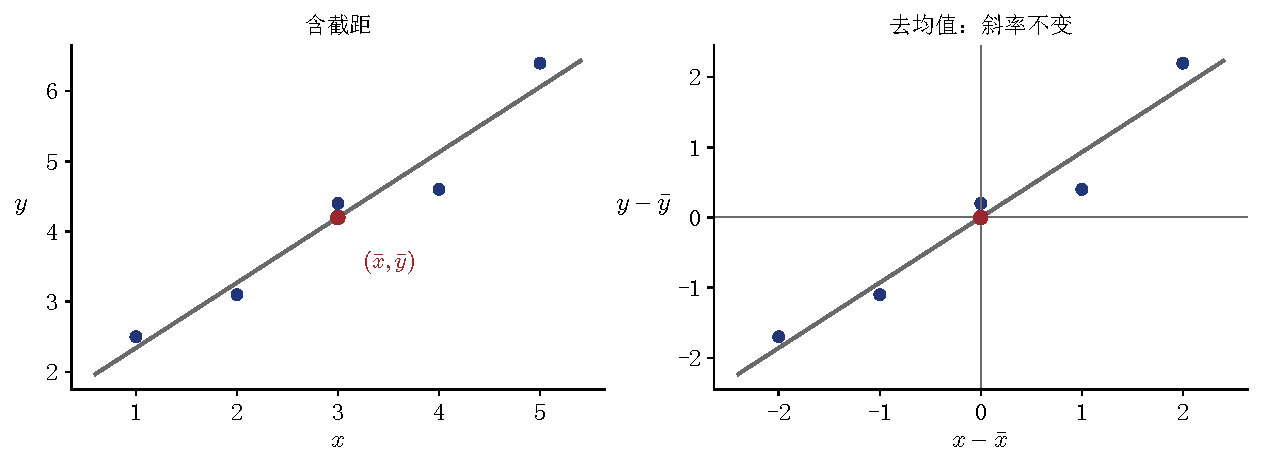
\includegraphics[width=.95\linewidth]{demeaning.pdf}
\caption{去均值将样本均值点移到原点，同时保留拟合斜率。本图采用示意观测。}
\label{fig:demeaning}
\end{figure}

\paragraph{原稿页底重复的例式（保留可见内容）.}
扫描页底再次写出了例式
\[\wage=\beta_0+\beta_1\educ+u,\]
并列出智力、家庭背景、经验和培训等未观测因素。它们仍与第 2 周的外生性讨论相关。此处不推测扫描可见范围之外的后续内容。

\subsection{OLS 公式：按补充推导页再次保留}
\sourcepage{3}{6}{补充推导页}
含截距时，
\[\hat\beta_1=\frac{\sum_i(x_i-\bar x)(y_i-\bar y)}{\sum_i(x_i-\bar x)^2},
\qquad\hat\beta_0=\bar y-\hat\beta_1\bar x.\]
不含截距时，
\begin{align*}
\frac{d}{db_1}\sum_i(y_i-b_1x_i)^2&=-2\sum_i x_i(y_i-b_1x_i),\\
\sum_i x_iy_i-\check\beta_1\sum_i x_i^2&=0,\\
\check\beta_1&=\frac{\sum_i x_iy_i}{\sum_i x_i^2}.
\end{align*}

\paragraph{为什么去均值有效？}
令 $x_i^*=x_i-\bar x$、$y_i^*=y_i-\bar y$，将 $y_i^*$ 对 $x_i^*$ 作无截距回归：
\[\hat\gamma=\frac{\sum_i x_i^*y_i^*}{\sum_i(x_i^*)^2}
=\frac{\sum_i(x_i-\bar x)(y_i-\bar y)}{\sum_i(x_i-\bar x)^2}=\hat\beta_1.\]
因此，就斜率而言，含截距 OLS $\Longleftrightarrow$ 去均值后的无截距 OLS。样本均值点变为 $(0,0)$，拟合线不发生旋转。

\paragraph{去均值就是对常数项回归后取残差。}
在仅含截距的回归 $y_i=b_0+e_i$ 中，
\[\frac{d}{db_0}\sum_i(y_i-b_0)^2=-2\sum_i(y_i-b_0)=0
\quad\Longrightarrow\quad\hat b_0=\bar y.\]
残差为 $y_i-\bar y$。同理，将 $x_i$ 对常数项回归，得到残差 $x_i-\bar x$。

\subsection{剔除线性影响：FWL 定理}
\label{sec:fwl-week3}
对于 $y_i=\beta_0+\beta_1x_i+\beta_2z_i+u_i$，原稿给出的三个步骤为：
\begin{enumerate}
\item 将 $y$ 对 $(1,z)$ 回归，得到残差 $r_{yi}$。
\item 将 $x$ 对 $(1,z)$ 回归，得到残差 $r_{xi}$。
\item 将 $r_y$ 对 $r_x$ 作无截距回归。
\end{enumerate}
结果为
\[\hm{\hat\beta_1=\frac{\sum_i r_{xi}r_{yi}}{\sum_i r_{xi}^2}}.\]
去均值是上述方法的一个特例：被剔除影响的变量只有常数项。这保留了原稿对两种方法之间联系的说明。

\section{无截距 OLS 的性质}
\sourcepage{3}{7}{3/6}
\label{sec:rto-properties}
回到过原点回归的目标函数，以及唯一系数对应的一阶条件：
\[\min_{b_1}\sum_i(y_i-b_1x_i)^2,\qquad
-2\sum_i x_i(y_i-\check\beta_1x_i)=0
\quad\Longrightarrow\quad\sum_i x_i\check u_i=0.\]
模型没有截距系数，因此也没有对截距求导的一阶条件。

\paragraph{性质一：残差均值不一定为零。}
模型不再强制 $\sum_i\check u_i=0$。某些特殊样本中它可以成立，但并无一般保证。

\paragraph{性质二：正交性仍成立，但协方差未必为零。}
仍有 $\sum_i x_i\check u_i=0$。然而，
\[\Cov_n(x,\check u)=\frac1n\sum_i x_i\check u_i-\bar x\bar{\check u}
=-\bar x\bar{\check u},\]
这一协方差一般不为零。\red{不能在无截距时把“内积为零”直接写成“样本不相关”。}\corr{rto-covariance}

\paragraph{性质三：样本均值点未必位于拟合线上。}
对 $y_i=\check\beta_1x_i+\check u_i$ 取平均，得
\[\bar y=\check\beta_1\bar x+\bar{\check u}.\]
因此，$\bar y=\check\beta_1\bar x$ 一般不成立。含截距时则由 $\bar{\hat u}=0$ 得到 $\bar y=\bar{\hat y}$。

\subsection[中心化判定系数可能为负]{中心化 $R^2$ 可能为负}
沿用 TSS 与 ESS 的中心化定义，有
\begin{equation}\label{eq:rto-cross-term}
\TSS=\ESS+\RSS+2\sum_i\check u_i(\hat y_i-\bar y).
\end{equation}
对于过原点拟合，$\sum_i\check u_i\hat y_i=0$，但 $\sum_i\check u_i$ 未必为零，因此交叉项不一定消失。\corr{rto-cross-term}
中心化统计量
\[R_c^2=1-\frac{\RSS}{\TSS}\]
可以为负：这意味着按平方误差衡量，强制过原点的拟合线比仅含均值的水平线 $\bar y$ 拟合得更差。
\begin{figure}[H]
\centering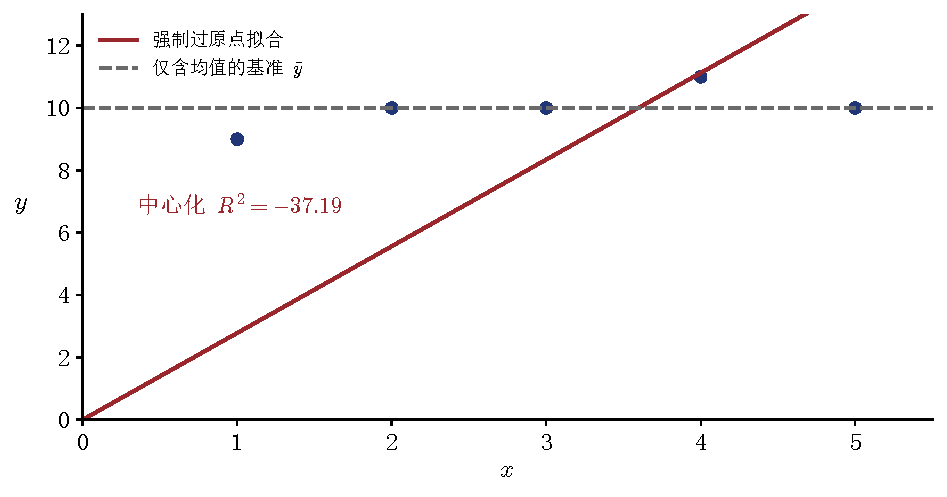
\includegraphics[width=.8\linewidth]{through_origin_negative_r2.pdf}
\caption{过原点拟合差于仅含均值的基准。示意数据 $x=(1,2,3,4,5)$、$y=(9,10,10,11,10)$ 产生了图中实际计算的负中心化 $R^2$。}
\label{fig:negative-r2}
\end{figure}
\added{某些软件对无截距模型报告\emph{非中心化}统计量 $R_u^2=1-\RSS/\sum_i y_i^2$。它以零为基准，而不是以 $\bar y$ 为基准，因此不能与含截距模型通常采用的中心化 $R^2$ 直接比较。}\corr{rto-r2}

\subsection*{本章小结}
\addcontentsline{toc}{subsection}{本章小结}
\begin{itemize}
\item 含截距时，OLS 残差的均值为零，与已纳入的回归变量在样本中正交，并有 TSS $=$ ESS $+$ RSS。
\item 在相同数据上对嵌套模型增加回归变量，普通 $R^2$ 不会下降，但调整 $R^2$ 可以下降。
\item 去均值与 FWL 保留完整模型中相应的斜率。省略截距会改变均值、协方差和中心化 $R^2$ 的性质。
\end{itemize}

\chapter{OLS 估计的无偏性}
\label{ch:week4}
\section{简单 OLS：概念、假设与定理}
\sourcepage{4}{1}{4/1}
\label{sec:unbiasedness-concept}
学习目标：
\begin{enumerate}
\item 陈述保证\hy{有限样本无偏性}的假设。
\item 用经济语言解释零条件均值。
\item 判断常见情形下遗漏变量偏误的方向。
\end{enumerate}
\subsection{估计与拟合优度回顾}
\[y=\beta_0+\beta_1x+u,\qquad
\hat y=\hat\beta_0+\hat\beta_1x,\]
\[\hat\beta_1=\frac{\Cov_n(x,y)}{\Var_n(x)},\qquad
\hat\beta_0=\bar y-\hat\beta_1\bar x,\qquad
R^2=\frac{\ESS}{\TSS}=1-\frac{\RSS}{\TSS}.\]
此处的 $R^2$ 恒等式要求模型含截距，且 TSS 为正。

\subsection{总体参数与估计量}
\begin{description}
\item[$\beta_j$。]固定但未知的总体参数。
\item[$\hat\beta_j$。]由随机样本计算的估计量。在观测样本之前，它是随机变量，会随样本改变，具有抽样分布；相应的矩在存在时才有定义。
\end{description}
在某个具体样本中，估计值可能高于或低于 $\beta_j$；并不要求它等于真值，也不能一般地预期每次都会相等。\corr{estimator-estimate}

\begin{definition}[无偏估计量]
若 $\theta$ 的估计量 $\hat\theta$ 的期望存在，并且
\[\hm{\E[\hat\theta]=\theta}.\]
则称该估计量\hy{无偏}。对于 OLS，我们寻找使 $\E[\hat\beta_0]=\beta_0$ 与 $\E[\hat\beta_1]=\beta_1$ 成立的条件。
\end{definition}
在重复抽样中，估计量的期望等于真实总体参数。在任意一个样本中，估计值仍可能明显偏离真值。\blue{无偏性描述重复抽样的平均表现，不保证某一次估计恰好正确，也不保证估计误差很小。}

\subsection{假设概览}
\begin{enumerate}[label=SLR\arabic*.]
\item 对参数线性：$y=\beta_0+\beta_1x+u$。
\item 随机抽样：$\{(x_i,y_i):i=1,\ldots,n\}$ 是来自总体模型的独立同分布观测。
\item 样本存在变异：$S_{xx}=\sum_i(x_i-\bar x)^2>0$。
\item 零条件均值：$\E[u\mid x]=0$。
\end{enumerate}
\added{若要陈述无条件无偏性，还须假设 OLS 估计量几乎处处有定义，且下文使用的期望存在。这里的均值无偏结论不要求误差正态分布，也不要求同方差。}

\subsection{简单 OLS 假设的详细说明}
\sourcepage{4}{2}{4/2}
\paragraph{SLR1：对参数线性。}
\[\hy{$y=\beta_0+\beta_1x+u$}.\]
未知系数以线性形式进入模型。可以对已观测变量作变换，而不必使模型对参数变为非线性。

\paragraph{SLR2：随机抽样。}
每个观测满足 $y_i=\beta_0+\beta_1x_i+u_i$。观测对 $(x_i,y_i)$ 在不同 $i$ 之间相互独立且同分布。因此，对 $i\ne j$，$u_i=y_i-\beta_0-\beta_1x_i$ 与 $u_j$ 独立；但这并不表示 $u_i$ 与其自身的回归变量 $x_i$ 独立。
\begin{figure}[htbp]
\centering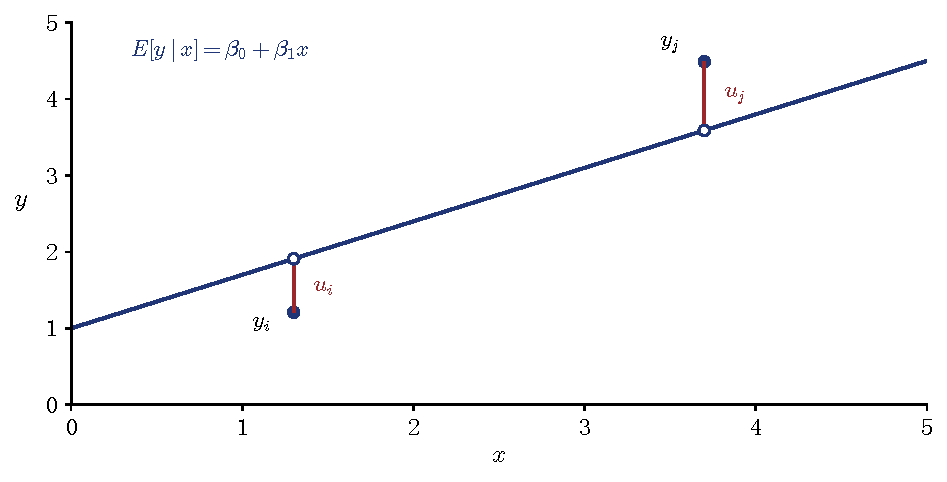
\includegraphics[width=.79\linewidth]{population_errors.pdf}
\caption{总体误差是观测值偏离条件均值的垂直距离，不是相对于估计回归线的残差。本图沿用原稿中的两个观测点示意，点的位置不代表真实数据。}
\label{fig:population-errors}
\end{figure}

\paragraph{SLR3：回归变量存在变异。}
观测到的 $x_i$ 不能全部取相同值：
\[\hy{$S_{xx}=\sum_i(x_i-\bar x)^2>0$}.\]
若所有 $x_i$ 都相同，斜率公式的分母为零，无法分别确定截距和斜率。

\paragraph{SLR4：零条件均值。}
\[\hy{$\E[u_i\mid x_i]=0$}\qquad(i=1,\ldots,n).\]
解释变量取任何值时，未观测因素的条件平均值均为零。在独立抽样下，这还意味着
\[\E[u_i\mid\mathcal X]=0,\qquad\mathcal X=(x_1,\ldots,x_n),\]
因为给定 $x_i$ 后，其他观测的回归变量不再提供有关 $u_i$ 的额外信息。证明中须以\emph{整个已观测样本设计}为条件，因为抽样前 $S_{xx}$ 是随机的。\corr{conditioning}

\begin{theorem}[简单 OLS 的无偏性]\label{thm:simple-unbiased}
在 SLR1--SLR4 及前述存在性条件成立时，
\[\E[\hat\beta_0\mid\mathcal X]=\beta_0,\qquad
\E[\hat\beta_1\mid\mathcal X]=\beta_1.\]
因此，$\E[\hat\beta_0]=\beta_0$，且 $\E[\hat\beta_1]=\beta_1$。
\end{theorem}

\subsection{斜率的无偏性证明}
逐步展开斜率公式：
\begin{align}
\hat\beta_1
&=\frac{\sum_i(x_i-\bar x)(y_i-\bar y)}{S_{xx}}
=\frac{\sum_i(x_i-\bar x)y_i}{S_{xx}}\notag\\
&=\frac{\sum_i(x_i-\bar x)(\beta_0+\beta_1x_i+u_i)}{S_{xx}}\notag\\
&=\frac{\beta_0\sum_i(x_i-\bar x)
+\beta_1\sum_i(x_i-\bar x)x_i+\sum_i(x_i-\bar x)u_i}{S_{xx}}.\label{eq:slope-expansion}
\end{align}
注意 $\sum_i(x_i-\bar x)=0$，并且
\begin{align*}
S_{xx}&=\sum_i(x_i^2-2x_i\bar x+\bar x^2)
=\sum_i x_i^2-n\bar x^2\\
&=\sum_i x_i(x_i-\bar x).
\end{align*}
因此，
\begin{equation}\label{eq:slope-error}
\hm{\hat\beta_1=\beta_1+\frac{\sum_i(x_i-\bar x)u_i}{S_{xx}}}.
\end{equation}
\begin{align*}
\E[\hat\beta_1\mid\mathcal X]
&=\beta_1+\frac{\sum_i(x_i-\bar x)\E[u_i\mid\mathcal X]}{S_{xx}}\\
&=\beta_1.
\end{align*}
最后，$\E[\hat\beta_1]=\E\{\E[\hat\beta_1\mid\mathcal X]\}=\beta_1$。\red{不能在无条件期望中直接把随机分母 $S_{xx}$ 提到期望外。}\corr{conditioning}

\subsection{截距的无偏性证明：考试提示}
\sourcepage{4}{3}{4/3}
\label{sec:intercept-proof}
对模型取样本平均，有
\[\bar y=\beta_0+\beta_1\bar x+\bar u,\qquad
\bar u=\frac1n\sum_i u_i.\]
将其代入 $\hat\beta_0=\bar y-\hat\beta_1\bar x$：
\[\hat\beta_0=\beta_0+(\beta_1-\hat\beta_1)\bar x+\bar u.\]
于是，
\begin{align*}
\E[\hat\beta_0\mid\mathcal X]
&=\beta_0+\bar x\bigl(\beta_1-\E[\hat\beta_1\mid\mathcal X]\bigr)
+\E[\bar u\mid\mathcal X]\\
&=\beta_0+\bar x(\beta_1-\beta_1)+0=\beta_0.
\end{align*}
$\bar u$ 项前应为\emph{加号}；手写证明中间一行出现了不一致的减号，此处已更正。\corr{intercept-sign}
再由迭代期望法则，得 $\E[\hat\beta_0]=\beta_0$。

\subsection{讨论：假设不成立会怎样？}
\blue{原稿在此处另有课堂时间标记：15 分钟。}
\begin{description}
\item[SLR1：对参数线性。]若模型对未知系数非线性，就超出了这里的线性 OLS 证明范围。\blue{非线性参数与变量的非线性变换要区分。}
\item[SLR2：随机抽样。]原稿列举了时间序列中的序列相关（自相关）、不具代表性的样本和观测间的溢出效应。这些情况可能违背所述独立同分布设定，或引发样本代表性与模型设定问题。但它们本身\emph{不能}证明每个 OLS 系数都有偏；还必须另行检查条件均值限制。\corr{violations}
\item[SLR3：样本变异。]若 $S_{xx}=0$，简单回归的斜率便无法与截距分别识别。
\item[SLR4：零条件均值。]在观测性研究中，遗漏因素可能与回归变量相关。若 $\Cov(x,u)\ne0$，ZCM 不可能成立。但 ZCM 比零协方差更强：$\Cov(x,u)=0$ 不能推出 $\E[u\mid x]=0$。单凭 ZCM 失败，也不能保证每种设计下都必然存在非零的有限样本偏差。\corr{zcm-covariance}
\end{description}
\added{原稿中的协方差恒等式为
\[\Cov(x,u)=\E[xu]-\E[x]\E[u].\]
在相应矩存在时，ZCM 同时推出 $\E[u]=0$ 与 $\E[xu]=0$。反方向一般不成立。}

\section{多元 OLS：假设与定理}
\sourcepage{4}{4}{4/5}
\label{sec:multiple-unbiased}
\subsection{MLR1：对参数线性}
总体模型为
\[y=\beta_0+\beta_1x_1+\beta_2x_2+\cdots+\beta_kx_k+u.\]
系数 $\beta_0,\ldots,\beta_k$ 是所关心的未知常数；$u$ 为误差项。

\subsection{MLR2：随机抽样}
从该总体模型取得 $n$ 个独立同分布的观测向量
\[\{(x_{1i},\ldots,x_{ki},y_i):i=1,\ldots,n\}\]
因此，$y_i=\beta_0+\sum_{j=1}^k\beta_jx_{ji}+u_i$。

\subsection{MLR3：不存在完全共线性}
包含截距列的样本设计矩阵具有满列秩。除截距外，任何回归变量都不是常数，也不存在某一列是其他列的精确线性组合。\blue{相关可以存在；完全线性的重复信息会使单独系数无法识别。}

\begin{example}[完全共线性]
保留原稿中的所有例子：
\begin{enumerate}
\item 常数回归变量：模型已含截距，却又加入 $x_1=10$。
\item 精确倍数或仿射关系：$x_1=2x_2$，或 $x_1=a+bx_2$。
\item 精确线性组合：$x_3=x_1+x_2$。
\end{enumerate}
\begin{figure}[htbp]
\centering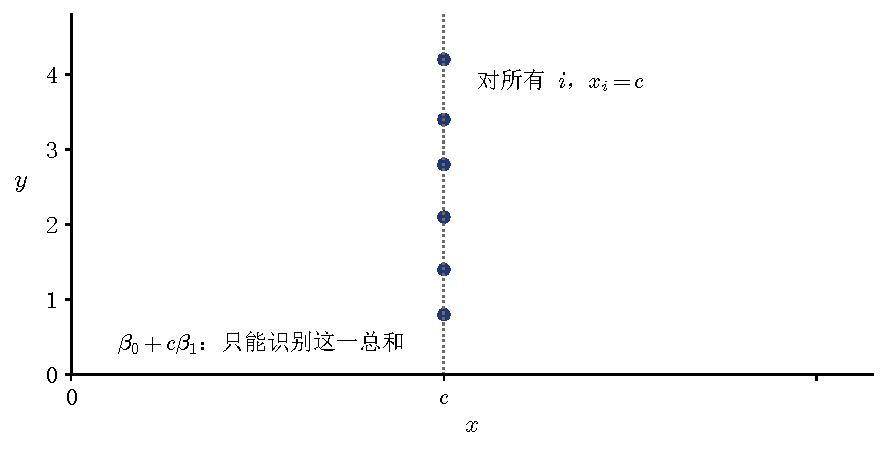
\includegraphics[width=.72\linewidth]{no_sample_variation.pdf}
\caption{若每个观测均有 $x_i=c$，只能识别 $\beta_0+c\beta_1$。本图以示意点重现原稿中 $x$ 为常数的情形。}
\label{fig:no-variation}
\end{figure}
若回归已包含 $\ln(\mathrm{income})$，再加入 $2\ln(\mathrm{income})$ 会造成完全共线性。同样，若总支出 $=$ 支出 A $+$ 支出 B，则同时纳入这三个变量也会造成完全共线性。

仅保留支出 A 与 B、删去它们的精确总和，并不会因此产生上述特定的共线关系。以下模型
\[y=\beta_0+\beta_1\ln(\mathrm{income})
+\beta_2[\ln(\mathrm{income})]^2+u\]
并\emph{不自动}具有完全共线性：变量的平方一般不是其水平值的仿射变换。\blue{它对变量可以非线性，但对参数仍线性。}不过，在取值种类过少等特殊样本中，设计矩阵仍可能不满秩。\corr{collinearity}
\end{example}


\subsection{MLR4：零条件均值}
\sourcepage{4}{5}{4/6}
\[\hm{\E[u\mid x_1,x_2,\ldots,x_k]=0}.\]
解释变量不能系统地预测误差的条件均值。在本笔记的术语中，这称为均值外生性条件。\red{它推出与误差不相关；仅仅不相关不足以推出这个条件。}\corr{zcm-covariance}
原稿区分了外生回归变量与内生回归变量。在结构模型中，若回归变量与 $u$ 中遗漏的决定因素相关，就可能存在内生性；与\emph{拟合残差}的样本协方差为零，不能排除这一问题。

\begin{theorem}[多元 OLS 的无偏性]\label{thm:multiple-unbiased}
在 MLR1--MLR4 成立、样本设计矩阵几乎处处满秩且相关期望存在时，
\[\E[\hat\beta_j\mid\mathcal X]=\beta_j,
\qquad\E[\hat\beta_j]=\beta_j,\qquad j=0,1,\ldots,k,\]
其中，$\mathcal X$ 表示整个已观测回归变量矩阵。
\end{theorem}

\subsection{利用剔除线性影响进行证明}
\label{sec:fwl-week4}
固定一个回归变量 $x_j$。按原稿的方法，将它对常数项及全部其他回归变量回归：
\begin{equation}\label{eq:auxiliary-j}
x_{ji}=\hat\delta_0+\sum_{\ell\ne j}\hat\delta_\ell x_{\ell i}+\hat r_{ji}.
\end{equation}
\blue{不同样本会有不同的辅助回归系数和残差。给定整组 $\mathcal X$，这些量都是已确定的。}
辅助回归的正规方程给出
\[\sum_i\hat r_{ji}=0,\qquad
\sum_i x_{\ell i}\hat r_{ji}=0\quad(\ell\ne j).\]
定义\emph{辅助回归}的残差平方和
\[S_{r_jr_j}=\sum_i\hat r_{ji}^{\,2}>0.
\]
这就是原稿记作“$\RSS_j$”的量，应与因变量回归的残差平方和区分。由于 $x_{ji}$ 等于其辅助回归拟合部分加上 $\hat r_{ji}$，有
\[\sum_i\hat r_{ji}x_{ji}=\sum_i\hat r_{ji}^{\,2}=S_{r_jr_j}.
\]
FWL 的单侧系数形式给出
\begin{align}
\hat\beta_j
&=\frac{\Cov_n(\hat r_j,y)}{\Var_n(\hat r_j)}
=\frac{\sum_i\hat r_{ji}y_i}{S_{r_jr_j}}\notag\\
&=\frac{\sum_i\hat r_{ji}\left(\beta_0+\sum_{\ell=1}^k\beta_\ell x_{\ell i}+u_i\right)}{S_{r_jr_j}}\notag\\
&=\hm{\beta_j+\frac{\sum_i\hat r_{ji}u_i}{S_{r_jr_j}}}.\label{eq:multiple-slope-error}
\end{align}
其余回归变量项都因辅助回归的正交性而消失。取条件期望，得
\[\E[\hat\beta_j\mid\mathcal X]
=\beta_j+\frac{\sum_i\hat r_{ji}\E[u_i\mid\mathcal X]}{S_{r_jr_j}}
=\beta_j.\]
由迭代期望法则，即可证明每个斜率的无条件无偏性。
\added{截距可由下式处理：
\[\hat\beta_0=\bar y-\sum_{j=1}^k\hat\beta_j\bar x_j
=\beta_0+\bar u+\sum_{j=1}^k(\beta_j-\hat\beta_j)\bar x_j.\]
给定 $\mathcal X$ 后，每个 $\bar x_j$ 都是固定的；利用斜率的结论及 $\E[\bar u\mid\mathcal X]=0$，得到 $\E[\hat\beta_0\mid\mathcal X]=\beta_0$。}

\section{假设汇总与无偏性}
\sourcepage{4}{6}{4/7}
\label{sec:assumptions-summary}
\paragraph{核心：控制其他因素。}
多元回归的核心能力是通过 FWL 排除其他已观测因素的线性影响，识别某一自变量剩余变化与结果的关系。\blue{“纯净影响”的因果说法仍依赖适当的模型与外生性，不能仅由控制操作保证。}

\paragraph{无偏性的本质：重复抽样的平均性质.}
单次抽样的具体估计是一个已经实现的数值；生成这些数值的 OLS 估计程序才有统计意义上的无偏性。

\subsection{四项假设的并列比较}
\begin{center}
\small\renewcommand{\arraystretch}{1.35}
\begin{tabular}{P{3.1cm}P{5.35cm}P{6.3cm}}
\toprule
假设 & 简单回归 & 多元回归\\
\midrule
对参数线性 & $y=\beta_0+\beta_1x+u$ & $y=\beta_0+\sum_{j=1}^k\beta_jx_j+u$\\
随机抽样 & 独立同分布的观测对 $(x_i,y_i)$ & 独立同分布的观测向量 $(x_{1i},\ldots,x_{ki},y_i)$\\
样本秩 & $\sum_i(x_i-\bar x)^2>0$ & 含常数列在内的设计矩阵各列之间，不存在精确线性关系\\
零条件均值 & $\E[u\mid x]=0$ & $\E[u\mid x_1,\ldots,x_k]=0$\\
\bottomrule
\end{tabular}
\end{center}

\begin{example}[某次教育回报率估计]\label{ex:unbiased-number}
原稿给出
\[\widehat{\ln(\wage)}
=0.284+0.092\educ+0.0041\,\mathrm{exper}+0.022\,\mathrm{tenure}.\]
若 MLR1--MLR4 成立，能否说“$9.2\%$ 是教育回报率的无偏估计”？

\red{无偏性属于估计量的性质。}数值 $0.092$ 是某一次估计的实现值。准确表述是：在所述假设下，对数工资方程中教育系数的 OLS 估计量无偏；它在本样本中的实现值为 $0.092$。

原稿中的“$9.2\%$”是教育年限增加一年时的近似百分比解释。保持误差不变时，精确的百分比变换为
\[100(e^{0.092}-1)\simeq9.64\%.
\]
\added{即使 $\hat\beta$ 是 $\beta$ 的无偏估计量，非线性变换 $e^{\hat\beta}-1$ 也未必是 $e^\beta-1$ 的无偏估计量。此外，拟合对数工资本身并不能识别教育的因果回报，也不能直接给出工资水平值的条件均值。}\corr{unbiased-log}
\end{example}

\section{模型设定与偏误}
\sourcepage{4}{7}{4/8}
\label{sec:model-specification}
这里区分两种模型设定：\hy{过度设定}，即加入无关变量；\hy{不足设定}，即遗漏相关变量。

\subsection{加入无关变量}
从以下模型出发：
\[y=\beta_0+\beta_1x_1+\beta_2x_2+u.\]
现在估计一个额外包含 $x_3$ 的模型，其总体系数 $\beta_3=0$。扩充后的样本设计仍须满秩，即 $x_3$ 不能是已有设计矩阵各列的精确线性组合。

若\emph{扩充后}的外生性条件成立，
\[\E[u\mid x_1,x_2,x_3]=0,
\]
则完整模型中的 OLS 估计量仍无偏：
\[\E[\hat\beta_j]=\beta_j\quad(j=0,1,2),\qquad
\E[\hat\beta_3]=0.
\]
\red{但仅有 $\E[u\mid x_1,x_2]=0$，并不能推出 $\E[u\mid x_1,x_2,x_3]=0$。}加入一个与误差相关的回归变量，会改变条件均值限制。某个系数为零，本身不能证明该新增控制变量具有外生性。\corr{irrelevant-exogeneity}

\added{在同方差、固定设计模型下，若加入无关变量减少了原有某个回归变量的残差变异，则该变量斜率的真实条件方差弱增，即不会下降。这不保证严格增加，也不保证某一次计算出的估计标准误一定上升。原稿中的“方差增加”须附带这些限定。}\corr{irrelevant-variance}

\subsection{遗漏相关变量}
\label{sec:ovb-sample}
设真实的长模型为
\[y_i=\beta_0+\beta_1x_i+\beta_2z_i+u_i,\qquad
\E[u_i\mid x_i,z_i]=0.\]
其拟合形式为
\[y_i=\hat\beta_0+\hat\beta_1x_i+\hat\beta_2z_i+\hat u_i.
\]
若 $z$ 未被观测或被遗漏，短回归将 $y$ 对 $(1,x)$ 回归：
\[y_i=\hat{\tilde\beta}_0+\hat{\tilde\beta}_1x_i+\hat v_i,
\qquad v_i=\beta_2z_i+u_i\ \text{（结构方程中的误差）}.
\]
当遗漏部分与 $x$ 相关时，遗漏一个相关变量才会影响 $x$ 的斜率；仅仅“该变量影响因变量”还不够。\corr{omitting-relevant}

\paragraph{短回归与长回归的精确样本恒等式。}
精确的样本关系为
\begin{equation}\label{eq:sample-ovb}
\hm{\hat{\tilde\beta}_1=\hat\beta_1+\hat\beta_2\hat\delta_1},
\end{equation}
其中，$\hat\delta_1$ 来自辅助 OLS 回归
\[z_i=\hat\delta_0+\hat\delta_1x_i+\hat r_i,
\qquad
\hat\delta_1=\frac{\sum_i(x_i-\bar x)(z_i-\bar z)}{S_{xx}}.
\]
首先，长模型残差与 $x$ 及常数项在样本中正交：
\begin{align*}
\sum_i(x_i-\bar x)(\hat u_i-\bar{\hat u})
&=\sum_i x_i\hat u_i-\bar x\sum_i\hat u_i\\
&=0.
\end{align*}
将去均值后的长模型拟合方程代入短回归斜率公式，得
\begin{align*}
\hat{\tilde\beta}_1
&=\frac{\sum_i(x_i-\bar x)(y_i-\bar y)}{S_{xx}}\\
&=\frac{\sum_i(x_i-\bar x)\left[\hat\beta_1(x_i-\bar x)
+\hat\beta_2(z_i-\bar z)+(\hat u_i-\bar{\hat u})\right]}{S_{xx}}\\
&=\hat\beta_1+\hat\beta_2\frac{\sum_i(x_i-\bar x)(z_i-\bar z)}{S_{xx}}+0\\
&=\hat\beta_1+\hat\beta_2\hat\delta_1.
\end{align*}
这是同一个具体样本中的代数恒等式，此处尚未取期望。

\subsection{期望偏差：哪些量是随机的？}
\sourcepage{4}{8}{4/9}
\label{sec:ovb-expectation}
现在令 $\mathcal X$ 包含样本中的全部 $x_i$ 与 $z_i$。在有效的长模型下，
\[\E[\hat\beta_1\mid\mathcal X]=\beta_1,
\qquad\E[\hat\beta_2\mid\mathcal X]=\beta_2.
\]
\emph{给定}这一设计后，辅助斜率 $\hat\delta_1$ 是固定的。因此，
\begin{align}
\E[\hat{\tilde\beta}_1\mid\mathcal X]
&=\E[\hat\beta_1+\hat\beta_2\hat\delta_1\mid\mathcal X]\notag\\
&=\hm{\beta_1+\beta_2\hat\delta_1},\label{eq:ovb-conditional}\\
\E[\hat{\tilde\beta}_1]
&=\beta_1+\beta_2\E[\hat\delta_1].\label{eq:ovb-unconditional}
\end{align}
等价地，保留原稿利用迭代期望的推导路线：
\begin{align*}
\E[\hat\beta_2\hat\delta_1]
&=\E\{\E[\hat\beta_2\hat\delta_1\mid\mathcal X]\}\\
&=\E\{\hat\delta_1\E[\hat\beta_2\mid\mathcal X]\}
=\beta_2\E[\hat\delta_1].
\end{align*}
\added{若要得到原稿中的有限样本表达式
\[\E[\hat{\tilde\beta}_1]=\beta_1+\beta_2\delta_1,\]
还需要 $\E[\hat\delta_1]=\delta_1$。一个充分的附加条件是辅助条件均值设定正确：
\[\E[z\mid x]=\delta_0+\delta_1x\]
并满足随机抽样、样本变异及所需可积性条件。仅将 $\delta_1$ 定义为总体投影斜率，并不能自动建立上述有限样本等式。}\corr{ovb-levels}

对于\emph{总体线性投影}，即使不增加上述线性条件均值假设，斜率差仍为
\[\tilde\beta_1-\beta_1=\beta_2\delta_1,
\qquad\delta_1=\frac{\Cov(x,z)}{\Var(x)}.
\]
在通常的一致性条件下，它也描述渐近的斜率差。总体与渐近结论不应和精确样本恒等式或有限样本期望混淆。

\subsection{遗漏变量偏误的方向}
若适用的斜率差或偏差为 $B=\beta_2\delta_1$，则
\begin{description}
\item[上偏。]$B>0$：短回归斜率高于目标 $\beta_1$。
\item[下偏。]$B<0$：短回归斜率低于目标 $\beta_1$。
\item[无偏差。]$B=0$，例如 $\beta_2=0$ 或 $\delta_1=0$。
\end{description}
当 $\Var(x)>0$ 时，$\delta_1$ 与 $\Cov(x,z)$ 同号。原稿的符号表写为
\begin{center}
\renewcommand{\arraystretch}{1.4}
\begin{tabular}{lcc}
\toprule
 & $\Cov(x,z)>0$ ($\delta_1>0$) & $\Cov(x,z)<0$ ($\delta_1<0$)\\
\midrule
$\beta_2>0$ & \hy{上偏} & 下偏\\
$\beta_2<0$ & 下偏 & \hy{上偏}\\
\bottomrule
\end{tabular}
\end{center}
\blue{该表直接适用于总体投影差；用于有限样本平均偏差时，应满足上一小节的附加条件。给定样本设计的偏差方向则由 $\hat\delta_1$ 决定。}

\paragraph{向零偏。}
当 $\beta_1$ 为正时，向零移动意味着下偏；当 $\beta_1$ 为负时，向零移动意味着上偏。若采用通常的衰减解释，偏移后的系数必须仍位于目标值与零之间。\red{方向正确但越过零，不能仅凭上偏或下偏就称为向零偏。}\corr{toward-zero}

\subsection*{本章小结}
\addcontentsline{toc}{subsection}{本章小结}
\begin{itemize}
\item 无偏性是估计量在重复抽样下的期望性质。
\item 样本设计满秩和零条件均值支撑了条件期望证明；仅有零协方差是更弱的条件。
\item 加入有效的无关控制变量可保持无偏性，但可能降低精度。遗漏既影响结果又与保留变量相关的回归变量，会改变斜率。
\item 应区分样本恒等式、条件偏差、无条件有限样本偏差与总体投影差。
\end{itemize}

\appendix
\ctexset{chapter={name={附录,},number=\Alph{chapter}}}
\chapter{原稿对应表}
\label{app:sources}
每行对应一页原始 PDF；点击正文页码可跳到该页内容开始的位置。跨页内容仍按原稿顺序衔接。所有 23 页均逐页查看，原稿中的重复讲解、例式和页底可见片段均保留。
第 4 周的手写页码跳号按用户说明属于练习安排，不标记为漏扫；不补写未提供的练习。第 2 周末页的手写页码以 PDF 第 8 页定位，避免猜写最后一位。
\small\renewcommand{\arraystretch}{1.25}
\begin{longtable}{P{1.05cm}P{.8cm}P{2.25cm}P{9.7cm}P{.9cm}}
\toprule 周次 & PDF & 手写页码 & 已整理内容 & 页码\\\midrule\endfirsthead
\toprule 周次 & PDF & 手写页码 & 已整理内容 & 页码\\\midrule\endhead
\bottomrule\endfoot
2 & 1 & 2/1 & 简单模型；其他条件不变；误差归一化；零条件均值；工资例题 & \hyperref[src:w2p1]{\pageref*{src:w2p1}}\\
2 & 2 & 2/2 & 总体回归函数推导；OLS 系数；相关与因果；截距；薪酬示意图 & \hyperref[src:w2p2]{\pageref*{src:w2p2}}\\
2 & 3 & 2/3 & 工资单位练习；安森的假设情景；得票与竞选支出练习 & \hyperref[src:w2p3]{\pageref*{src:w2p3}}\\
2 & 4 & 2/4 & 多元偏效应；相关的控制变量；平均绩点解释；安森与贝蒂 & \hyperref[src:w2p4]{\pageref*{src:w2p4}}\\
2 & 5 & 2/5 & 控制变量；能力；保持不变；单侧及一般 FWL 定理 & \hyperref[src:w2p5]{\pageref*{src:w2p5}}\\
2 & 6 & 2/6 & 短回归与长回归；系数相同的条件；舍入后的绩点方程 & \hyperref[src:w2p6]{\pageref*{src:w2p6}}\\
2 & 7 & 2/7 & 因变量与自变量单位变换；截距解释；样本协方差推导 & \hyperref[src:w2p7]{\pageref*{src:w2p7}}\\
2 & 8 & 末页，按 PDF 定位 & 水平值与对数的四类模型；百分比解释 & \hyperref[src:w2p8]{\pageref*{src:w2p8}}\\
3 & 1 & 3/1 & 误差与残差；简单 OLS 的三个样本性质；总体矩条件 & \hyperref[src:w3p1]{\pageref*{src:w3p1}}\\
3 & 2 & 3/2 & 三类平方和；交叉项证明；完全拟合；判定系数的相关解释 & \hyperref[src:w3p2]{\pageref*{src:w3p2}}\\
3 & 3 & 3/3 & 判定系数比较图；再次保留多元 OLS 性质及证明 & \hyperref[src:w3p3]{\pageref*{src:w3p3}}\\
3 & 4 & 3/4 & 增加回归变量；调整判定系数；绩点数值核算；三点提醒 & \hyperref[src:w3p4]{\pageref*{src:w3p4}}\\
3 & 5 & 3/5 & 过原点估计；去均值；均值点示意图；页底重复的工资例式 & \hyperref[src:w3p5]{\pageref*{src:w3p5}}\\
3 & 6 & 补充推导页 & 再次保留有无截距的公式；去均值；仅含常数项的回归；FWL & \hyperref[src:w3p6]{\pageref*{src:w3p6}}\\
3 & 7 & 3/6 & 再次保留过原点回归一阶条件；样本性质；协方差限制；负判定系数 & \hyperref[src:w3p7]{\pageref*{src:w3p7}}\\
4 & 1 & 4/1 & 学习目标；估计回顾；参数与估计量；无偏性；简单回归假设概览 & \hyperref[src:w4p1]{\pageref*{src:w4p1}}\\
4 & 2 & 4/2 & 简单回归假设详解；总体误差示意图；斜率无偏性的证明 & \hyperref[src:w4p2]{\pageref*{src:w4p2}}\\
4 & 3 & 4/3 & 考试提示中的截距证明；违背假设的后果及结论边界 & \hyperref[src:w4p3]{\pageref*{src:w4p3}}\\
4 & 4 & 4/5 & 多元回归前三项假设；常数自变量示意图；全部完全共线性例子 & \hyperref[src:w4p4]{\pageref*{src:w4p4}}\\
4 & 5 & 4/6 & 多元回归第四项假设；无偏性定理；辅助残差性质；FWL 期望证明 & \hyperref[src:w4p5]{\pageref*{src:w4p5}}\\
4 & 6 & 4/7 & 控制变量与无偏性回顾；假设对照表；某次对数工资估计 & \hyperref[src:w4p6]{\pageref*{src:w4p6}}\\
4 & 7 & 4/8 & 无关控制变量；遗漏相关变量；短长回归的精确样本恒等式 & \hyperref[src:w4p7]{\pageref*{src:w4p7}}\\
4 & 8 & 4/9 & 迭代期望偏误证明；附加条件；偏误方向与符号表 & \hyperref[src:w4p8]{\pageref*{src:w4p8}}\\
\end{longtable}\normalsize
\section*{复现与原件}
原始 PDF 和 BMO 模板副本保持原样；文件路径、字节数及 SHA256 校验值见项目中的 sources/manifest.json。矢量图和对应预览由同一 Python 脚本生成，数值检查记录另保存在 qa 目录。

\chapter{勘误与补充说明}

\label{app:errata}

正文直接采用正确写法；本附录记录实质修正及必要条件补充。原稿本来正确的结论不因列入此处而被视为错误；部分条目只是限制适用范围或明确记号。点原稿定位可返回正文；未删除原稿学习内容。

\section*{核对依据}

\begin{description}

\item[H1.] 汉森，\emph{计量经济学}，2010 年 1 月 10 日稿，第 2 章：条件均值、投影与解释。 \href{https://users.ssc.wisc.edu/~xshi28/Econometrics_Hansen.pdf}{大学网站公开的教材手稿}.

\item[H2.] 同一手稿，第 3.3 至 3.7 节及第 3.10 节：OLS 代数、残差回归与拟合优度。

\item[H3.] 同一手稿，第 4.3、4.4、4.11、4.12 节：条件无偏性、方差、共线性与遗漏变量。本笔记还明确推导了额外的有限样本限定条件。

\item[M.] 梅西大学， \href{https://r-resources.massey.ac.nz/161251/lectures/RegressionOrigin.html}{\emph{过原点回归}}: 中心化与非中心化拟合统计量的比较。

\item[计算.] 对原稿算式直接进行代数推导或数值运算；项目中包含可复现的数值核对。

\end{description}

外部材料仅用于核对数学与适用条件；本次排版模板仍是用户指定的旧 BMO 笔记。

\par\medskip\noindent\begin{minipage}{\linewidth}

\phantomsection\label{err:notation}

\textbf{C01. 总体、估计量与拟合值记号}\quad\textbf{原稿定位：}\hyperref[src:w2p4]{第 2 周，PDF 第 4 页}；\hyperref[src:w3p1]{第 3 周，PDF 第 1 页}。\quad\textbf{核对：}H1。\par

总体参数写作 $\beta_j$，样本估计写作 $\hat\beta_j$；总体误差 $u_i$ 与残差 $\hat u_i$ 分开。拟合值变化使用 $\Delta\hat y$，不将 $\hat\beta_j$ 直接写成总体参数。

\end{minipage}\par

\par\medskip\noindent\begin{minipage}{\linewidth}

\phantomsection\label{err:mean-normalisation}

\textbf{C02. 误差均值的归一化}\quad\textbf{原稿定位：}\hyperref[src:w2p1]{第 2 周，PDF 第 1 页}。\quad\textbf{核对：}H1。\par

令 $\varepsilon=u-\alpha$ 后，$\E[\varepsilon]=0$，而不是 $\varepsilon$ 处处等于零。截距变为 $\beta_0+\alpha$。该归一化本身不保证零条件均值。

\end{minipage}\par

\par\medskip\noindent\begin{minipage}{\linewidth}

\phantomsection\label{err:slope-correlation}

\textbf{C03. 斜率与相关系数的比例}\quad\textbf{原稿定位：}\hyperref[src:w2p2]{第 2 周，PDF 第 2 页}。\quad\textbf{核对：}H2。\par

样本简单 OLS 斜率为 $r_{xy}s_y/s_x$，不是 $r_{xy}s_x/s_y$；总体投影系数和样本系数不能混用。

\end{minipage}\par

\par\medskip\noindent\begin{minipage}{\linewidth}

\phantomsection\label{err:causality}

\textbf{C04. 相关与因果的边界}\quad\textbf{原稿定位：}\hyperref[src:w2p2]{第 2 周，PDF 第 2 页}；\hyperref[src:w2p4]{第 2 周，PDF 第 4 页}。\quad\textbf{核对：}H1。\par

保留“相关联”的措辞；控制变量、ZCM 或好的拟合度本身不能替代结构模型与可辩护的因果识别。截距在 $x=0$ 不可行时只是外推。

\end{minipage}\par

\par\medskip\noindent\begin{minipage}{\linewidth}

\phantomsection\label{err:wage-counterfactual}

\textbf{C05. 工资题中的单位与个体反事实}\quad\textbf{原稿定位：}\hyperref[src:w2p3]{第 2 周，PDF 第 3 页}。\quad\textbf{核对：}计算。\par

按原稿“千美元”复算：$5.58$、$-5.574$、$7.74$、$2.166$ 均使用同一单位。固定该人残差得到的是模型情景，并非保证的实际工资。未把看似异常的原题单位擅自改成美元。

\end{minipage}\par

\par\medskip\noindent\begin{minipage}{\linewidth}

\phantomsection\label{err:election}

\textbf{C06. 选举题的比例与金额}\quad\textbf{原稿定位：}\hyperref[src:w2p3]{第 2 周，PDF 第 3 页}。\quad\textbf{核对：}计算。\par

40\% 应输入 40，预测为 45.37\%；50\% 的预测阈值对应 支出占比 $>49.978448\ldots$。补齐在 B 支出 20 亿美元时 A 的支出阈值，区别预测过半与实际获胜。

\end{minipage}\par

\par\medskip\noindent\begin{minipage}{\linewidth}

\phantomsection\label{err:fwl-residual}

\textbf{C07. FWL 的单侧与双侧残差化}\quad\textbf{原稿定位：}\hyperref[src:w2p5]{第 2 周，PDF 第 5 页}；\hyperref[src:w4p5]{第 4 周，PDF 第 5 页}。\quad\textbf{核对：}H2。\par

只残差化自变量后回归原始 $y$，系数相同，但残差一般不等于原多元模型残差。对 $y$ 与该自变量同时排除其他回归量，才能同时得到相同系数与残差。

\end{minipage}\par

\par\medskip\noindent\begin{minipage}{\linewidth}

\phantomsection\label{err:ovb-levels}

\textbf{C08. 遗漏变量公式的三个层次}\quad\textbf{原稿定位：}\hyperref[src:w2p6]{第 2 周，PDF 第 6 页}；\hyperref[src:w4p8]{第 4 周，PDF 第 8 页}。\quad\textbf{核对：}H3。\par

保留样本恒等式 $\hat{\tilde\beta}_1=\hat\beta_1+\hat\beta_2\hat\delta_1$。给定整组设计时，偏差为 $\beta_2\hat\delta_1$；无条件有限样本偏差为 $\beta_2\E[\hat\delta_1]$。写成 $\beta_2\delta_1$ 还须有辅助斜率无偏等附加条件；总体投影差另行说明。

\end{minipage}\par

\par\medskip\noindent\begin{minipage}{\linewidth}

\phantomsection\label{err:unit-intercept}

\textbf{C09. 换单位时的截距与条件均值}\quad\textbf{原稿定位：}\hyperref[src:w2p7]{第 2 周，PDF 第 7 页}。\quad\textbf{核对：}计算。\par

总体截距的含义是 $\E[y\mid x=0]$，不是一般的 $\E[y]$；$y$ 乘以 $c$ 时截距也乘以 $c$。$x$ 乘以非零 $c$ 时斜率除以 $c$，截距不变。

\end{minipage}\par

\par\medskip\noindent\begin{minipage}{\linewidth}

\phantomsection\label{err:logs}

\textbf{C10. 有限变化与对数近似}\quad\textbf{原稿定位：}\hyperref[src:w2p8]{第 2 周，PDF 第 8 页}。\quad\textbf{核对：}计算。\par

将有限变化的近似与精确关系分开。水平值—对数模型为 $\beta_1\ln(x_1/x_0)$；对数—水平值模型的精确百分比为 $100(e^{\beta_1\Delta x}-1)$；对数—对数模型使用比例的幂。对数模型的系数仍保留原稿的局部百分比解释。

\end{minipage}\par

\par\medskip\noindent\begin{minipage}{\linewidth}

\phantomsection\label{err:sample-population}

\textbf{C11. 样本恒等式不是总体外生性的检验}\quad\textbf{原稿定位：}\hyperref[src:w3p1]{第 3 周，PDF 第 1 页}。\quad\textbf{核对：}H2。\par

残差和为零、与包含的回归量正交来自样本 OLS 一阶条件。不能从这些条件推出真实误差的 ZCM。总体均值关系用无帽参数，样本均值关系用样本系数。

\end{minipage}\par

\par\medskip\noindent\begin{minipage}{\linewidth}

\phantomsection\label{err:r2-degenerate}

\textbf{C12. 判定系数 的退化情形}\quad\textbf{原稿定位：}\hyperref[src:w3p2]{第 3 周，PDF 第 2 页}。\quad\textbf{核对：}H2。\par

补充 TSS 必须大于零。拟合值恒定时，普通 $R^2$ 可以为零，但相关系数因分母为零而未定义；此时不能直接用相关系数平方计算。

\end{minipage}\par

\par\medskip\noindent\begin{minipage}{\linewidth}

\phantomsection\label{err:r2-rss}

\textbf{C13. 高拟合度与 RSS 的比较}\quad\textbf{原稿定位：}\hyperref[src:w3p3]{第 3 周，PDF 第 3 页}。\quad\textbf{核对：}H2。\par

高 $R^2$ 表示较小的 RSS/TSS；不能跨不同样本或单位仅凭较高 $R^2$ 就认定绝对 RSS 更小。图中 0.94 和 0.64 均由新绘制的示意点实际计算。

\end{minipage}\par

\par\medskip\noindent\begin{minipage}{\linewidth}

\phantomsection\label{err:r2-monotonic}

\textbf{C14. 增加回归量时 判定系数 不减}\quad\textbf{原稿定位：}\hyperref[src:w3p4]{第 3 周，PDF 第 4 页}。\quad\textbf{核对：}H2。\par

原稿的“增加”改为“不下降，可以保持不变”，并注明必须是相同观测、相同因变量的嵌套 OLS 比较。不同缺失值样本不在该结论内。

\end{minipage}\par

\par\medskip\noindent\begin{minipage}{\linewidth}

\phantomsection\label{err:adjusted-meaning}

\textbf{C15. 调整判定系数 的提高条件}\quad\textbf{原稿定位：}\hyperref[src:w3p4]{第 3 周，PDF 第 4 页}。\quad\textbf{核对：}计算。\par

“变量有意义才提高”改写为残差均方必须下降；增加 $q$ 个回归量时，对应描述性的 偏 F 统计量 大于 1。这个阈值不是常规显著性检验，也不证明因果。

\end{minipage}\par

\par\medskip\noindent\begin{minipage}{\linewidth}

\phantomsection\label{err:demeaning}

\textbf{C16. 去均值与过原点回归}\quad\textbf{原稿定位：}\hyperref[src:w3p5]{第 3 周，PDF 第 5 页}；\hyperref[src:w3p6]{第 3 周，PDF 第 6 页}。\quad\textbf{核对：}H2。\par

是“去均值后无截距”的斜率等于“原始数据带截距”的斜率；不是任意无截距回归都等于带截距回归。原稿的两次推导均保留。

\end{minipage}\par

\par\medskip\noindent\begin{minipage}{\linewidth}

\phantomsection\label{err:rto-covariance}

\textbf{C17. 无截距时的正交与不相关}\quad\textbf{原稿定位：}\hyperref[src:w3p7]{第 3 周，PDF 第 7 页}。\quad\textbf{核对：}H2。\par

$\sum_i x_i\check u_i=0$ 仍成立，但 $\Cov_n(x,\check u)=-\bar x\bar{\check u}$ 一般不为零。原稿将两者等同的说法已改正。

\end{minipage}\par

\par\medskip\noindent\begin{minipage}{\linewidth}

\phantomsection\label{err:rto-cross-term}

\textbf{C18. 平方和分解的交叉项}\quad\textbf{原稿定位：}\hyperref[src:w3p7]{第 3 周，PDF 第 7 页}。\quad\textbf{核对：}H2。\par

交叉项应为 $2\sum_i\check u_i(\hat y_i-\bar y)$，其中是拟合值 $\hat y_i$。无截距时它不一定消失，因此不能一般地写 TSS=ESS+RSS。

\end{minipage}\par

\par\medskip\noindent\begin{minipage}{\linewidth}

\phantomsection\label{err:rto-r2}

\textbf{C19. 有截距与无截距 判定系数 的基准}\quad\textbf{原稿定位：}\hyperref[src:w3p7]{第 3 周，PDF 第 7 页}。\quad\textbf{核对：}M。\par

区分以样本均值为基准的 中心化判定系数 与以零为基准的 非中心化判定系数。前者在过原点回归中可以为负；两种统计量不能当作同一尺度直接比较。

\end{minipage}\par

\par\medskip\noindent\begin{minipage}{\linewidth}

\phantomsection\label{err:estimator-estimate}

\textbf{C20. 估计量与某次估计值}\quad\textbf{原稿定位：}\hyperref[src:w4p1]{第 4 周，PDF 第 1 页}。\quad\textbf{核对：}H3。\par

无偏性不要求某一次估计等于真值，也不声称每一次估计必定不等于真值。它是对重复抽样期望的限制，并需要相关期望存在。

\end{minipage}\par

\par\medskip\noindent\begin{minipage}{\linewidth}

\phantomsection\label{err:conditioning}

\textbf{C21. 无偏性证明的条件期望}\quad\textbf{原稿定位：}\hyperref[src:w4p2]{第 4 周，PDF 第 2 页}；\hyperref[src:w4p5]{第 4 周，PDF 第 5 页}。\quad\textbf{核对：}H3。\par

先给定整组样本设计，再将样本权重与分母作为常量提出条件期望。不能仅使用单个 $x_i$ 的条件，或在无条件期望中把随机分母当常数。注明样本满秩和期望存在。

\end{minipage}\par

\par\medskip\noindent\begin{minipage}{\linewidth}

\phantomsection\label{err:intercept-sign}

\textbf{C22. 截距证明的正负号}\quad\textbf{原稿定位：}\hyperref[src:w4p3]{第 4 周，PDF 第 3 页}。\quad\textbf{核对：}计算。\par

从总体模型取平均得到 $\bar y=\beta_0+\beta_1\bar x+\bar u$；因此截距展开式中的 $\bar u$ 应为加号。原稿中间一行的减号与其余推导不一致。

\end{minipage}\par

\par\medskip\noindent\begin{minipage}{\linewidth}

\phantomsection\label{err:violations}

\textbf{C23. 违背抽样假设的后果}\quad\textbf{原稿定位：}\hyperref[src:w4p3]{第 4 周，PDF 第 3 页}。\quad\textbf{核对：}H3。\par

保留时间序列相关、非代表性样本和溢出效应的例子；将它们与“必然产生 OLS 偏差”区分。需另查条件均值，不能仅凭违反独立同分布假设 就推出所有系数有偏。

\end{minipage}\par

\par\medskip\noindent\begin{minipage}{\linewidth}

\phantomsection\label{err:zcm-covariance}

\textbf{C24. ZCM 强于零协方差}\quad\textbf{原稿定位：}\hyperref[src:w4p3]{第 4 周，PDF 第 3 页}；\hyperref[src:w4p5]{第 4 周，PDF 第 5 页}。\quad\textbf{核对：}H1。\par

$\E[u\mid x]=0$ 推出零均值、零协方差；反方向不成立。总体误差不相关不足以保证有限样本无偏；与样本残差正交也不构成外生性的证据。

\end{minipage}\par

\par\medskip\noindent\begin{minipage}{\linewidth}

\phantomsection\label{err:collinearity}

\textbf{C25. 完全共线性与平方项}\quad\textbf{原稿定位：}\hyperref[src:w4p4]{第 4 周，PDF 第 4 页}。\quad\textbf{核对：}H3。\par

保留常数、倍数、仿射关系、总支出等例子。对数变量及其平方一般不自动完全共线，但特殊样本仍可能不满秩；“样本满秩所以总体一定如何”的措辞改为直接检查样本设计。

\end{minipage}\par

\par\medskip\noindent\begin{minipage}{\linewidth}

\phantomsection\label{err:unbiased-log}

\textbf{C26. 9.2\% 与无偏估计程序}\quad\textbf{原稿定位：}\hyperref[src:w4p6]{第 4 周，PDF 第 6 页}。\quad\textbf{核对：}H3。\par

改正 $\log(\widehat{wage})$ 与 $\widehat{\log(wage)}$ 的混用。0.092 是一个实现值；OLS 系数估计量的无偏不保证指数变换无偏。9.2\% 是近似，精确的固定误差变换约为 9.64\%。

\end{minipage}\par

\par\medskip\noindent\begin{minipage}{\linewidth}

\phantomsection\label{err:irrelevant-exogeneity}

\textbf{C27. 加入无关变量需要扩充后的外生性}\quad\textbf{原稿定位：}\hyperref[src:w4p7]{第 4 周，PDF 第 7 页}。\quad\textbf{核对：}H3。\par

不能从 $\E[u\mid x_1,x_2]=0$ 自动推出加入 $x_3$ 后条件均值仍为零。仅在扩充后满秩且继续满足 ZCM 等条件时，原有系数及零系数的 OLS 估计量才保持无偏。

\end{minipage}\par

\par\medskip\noindent\begin{minipage}{\linewidth}

\phantomsection\label{err:irrelevant-variance}

\textbf{C28. 无关控制变量与精度}\quad\textbf{原稿定位：}\hyperref[src:w4p7]{第 4 周，PDF 第 7 页}。\quad\textbf{核对：}H3。\par

将“估计方差必然上升”限定为同方差固定设计下，加入无关控制使相关真实条件方差弱增；不保证严格增加，也不保证每次实现的估计标准误增加。

\end{minipage}\par

\par\medskip\noindent\begin{minipage}{\linewidth}

\phantomsection\label{err:omitting-relevant}

\textbf{C29. 遗漏相关变量的条件}\quad\textbf{原稿定位：}\hyperref[src:w4p7]{第 4 周，PDF 第 7 页}。\quad\textbf{核对：}H3。\par

小节标题按内容改为 遗漏相关变量；遗漏变量系数非零并不足以保证目标斜率改变，还要看它与保留回归量的关系。误差、短回归残差、长回归残差分开。

\end{minipage}\par

\par\medskip\noindent\begin{minipage}{\linewidth}

\phantomsection\label{err:toward-zero}

\textbf{C30. 向零偏不能只看上偏或下偏}\quad\textbf{原稿定位：}\hyperref[src:w4p8]{第 4 周，PDF 第 8 页}。\quad\textbf{核对：}计算。\par

保留正系数下偏、负系数上偏的方向解释，但增加“不越过零”的限制。发生符号反转时不能仅按方向就称为通常意义的向零偏。

\end{minipage}\par

\end{document}
